%&preformat-disser
\RequirePackage[l2tabu,orthodox]{nag} % Раскомментировав, можно в логе получать рекомендации относительно правильного использования пакетов и предупреждения об устаревших и нерекомендуемых пакетах
% Формат А4, 14pt (ГОСТ Р 7.0.11-2011, 5.3.6)
\documentclass[a4paper,14pt,oneside,openany]{memoir}

%%%%%%%%%%%%%%%%%%%%%%%%%%%%%%%%%%%%%%%%%%%%%%%%%%%%%%%%%%%%%%%%%%%%%%%%%%%%%%%%
%%%% Файл упрощённых настроек шаблона, общих для диссертации и автореферата %%%%
%%%%%%%%%%%%%%%%%%%%%%%%%%%%%%%%%%%%%%%%%%%%%%%%%%%%%%%%%%%%%%%%%%%%%%%%%%%%%%%%

%%% Режим черновика %%%
\makeatletter
\@ifundefined{c@draft}{
  \newcounter{draft}
  \setcounter{draft}{0}  % 0 --- чистовик (максимальное соблюдение ГОСТ)
                         % 1 --- черновик (отклонения от ГОСТ, но быстрая
                         %       сборка итоговых PDF)
}{}
\makeatother

%%% Пометки в тексте %%%
\makeatletter
\@ifundefined{c@showmarkup}{
  \newcounter{showmarkup}
  \setcounter{showmarkup}{0}  % 0 --- скрыть пометки
                              % 1 --- показывать пометки
}{}
\makeatother

%%% Использование в pdflatex шрифтов не по-умолчанию %%%
\makeatletter
\@ifundefined{c@usealtfont}{
  \newcounter{usealtfont}
  \setcounter{usealtfont}{1}    % 0 --- шрифты на базе Computer Modern
                                % 1 --- использовать пакет pscyr, при его
                                %       наличии
                                % 2 --- использовать пакет XCharter, при наличии
                                %       подходящей версии
}{}
\makeatother

%%% Использование в xelatex и lualatex семейств шрифтов %%%
\makeatletter
\@ifundefined{c@fontfamily}{
  \newcounter{fontfamily}
  \setcounter{fontfamily}{1}  % 0 --- CMU семейство. Используется как fallback;
                              % 1 --- Шрифты от MS (Times New Roman и компания)
                              % 2 --- Семейство Liberation
}{}
\makeatother

%%% Библиография %%%
\makeatletter
\@ifundefined{c@bibliosel}{
  \newcounter{bibliosel}
  \setcounter{bibliosel}{1}   % 0 --- встроенная реализация с загрузкой файла
                              %       через движок bibtex8;
                              % 1 --- реализация пакетом biblatex через движок
                              %       biber
}{}
\makeatother

%%% Вывод типов ссылок в библиографии %%%
\makeatletter
\@ifundefined{c@mediadisplay}{
  \newcounter{mediadisplay}
  \setcounter{mediadisplay}{1}   % 0 --- не делать ничего; надписи [Текст] и
                                 %       [Эл. ресурс] будут выводиться только в ссылках с
                                 %       заполненным полем `media`;
                                 % 1 --- автоматически добавлять надпись [Текст] к ссылкам с
                                 %       незаполненным полем `media`; таким образом, у всех
                                 %       источников будет указан тип, что соответствует
                                 %       требованиям ГОСТ
                                 % 2 --- автоматически удалять надписи [Текст], [Эл. Ресурс] и др.;
                                 %       не соответствует ГОСТ
                                 % 3 --- автоматически удалять надпись [Текст];
                                 %       не соответствует ГОСТ
                                 % 4 --- автоматически удалять надпись [Эл. Ресурс];
                                 %       не соответствует ГОСТ
}{}
\makeatother

%%% Предкомпиляция tikz рисунков для ускорения работы %%%
\makeatletter
\@ifundefined{c@imgprecompile}{
  \newcounter{imgprecompile}
  \setcounter{imgprecompile}{0}   % 0 --- без предкомпиляции;
                                  % 1 --- пользоваться предварительно
                                  %       скомпилированными pdf вместо генерации
                                  %       заново из tikz
}{}
\makeatother
            % общие настройки шаблона
%%% Проверка используемого TeX-движка %%%
\newif\ifxetexorluatex   % определяем новый условный оператор (http://tex.stackexchange.com/a/47579)
\ifxetex
    \xetexorluatextrue
\else
    \ifluatex
        \xetexorluatextrue
    \else
        \xetexorluatexfalse
    \fi
\fi

\newif\ifsynopsis           % Условие, проверяющее, что документ --- автореферат

\usepackage{etoolbox}[2015/08/02]   % Для продвинутой проверки разных условий
\providebool{presentation}

\usepackage{comment}    % Позволяет убирать блоки текста (добавляет
                        % окружение comment и команду \excludecomment)

%%% Поля и разметка страницы %%%
\usepackage{pdflscape}  % Для включения альбомных страниц
\usepackage{geometry}   % Для последующего задания полей

%%% Математические пакеты %%%
\usepackage{amsthm,amsmath,amscd}   % Математические дополнения от AMS
\usepackage{amsfonts,amssymb}       % Математические дополнения от AMS
\usepackage{mathtools}              % Добавляет окружение multlined
\usepackage{xfrac}                  % Красивые дроби
\usepackage[
    locale = DE,
    list-separator       = {;\,},
    list-final-separator = {;\,},
    list-pair-separator  = {;\,},
    list-units           = single,
    range-units          = single,
    range-phrase={\text{\ensuremath{-}}},
    % quotient-mode        = fraction, % красивые дроби могут не соответствовать ГОСТ
    fraction-function    = \sfrac,
    separate-uncertainty,
    ]{siunitx}[=v2]                 % Размерности SI
\sisetup{inter-unit-product = \ensuremath{{}\cdot{}}}

% Кириллица в нумерации subequations
% Для правильной работы требуется выполнение сразу после загрузки пакетов
\patchcmd{\subequations}{\def\theequation{\theparentequation\alph{equation}}}
{\def\theequation{\theparentequation\asbuk{equation}}}
{\typeout{subequations patched}}{\typeout{subequations not patched}}

%%%% Установки для размера шрифта 14 pt %%%%
%% Формирование переменных и констант для сравнения (один раз для всех подключаемых файлов)%%
%% должно располагаться до вызова пакета fontspec или polyglossia, потому что они сбивают его работу
\newlength{\curtextsize}
\newlength{\bigtextsize}
\setlength{\bigtextsize}{13.9pt}

\makeatletter
%\show\f@size    % неплохо для отслеживания, но вызывает стопорение процесса,
                 % если документ компилируется без команды  -interaction=nonstopmode
\setlength{\curtextsize}{\f@size pt}
\makeatother

%%% Кодировки и шрифты %%%
\ifxetexorluatex
    \ifpresentation
        \providecommand*\autodot{} % quick fix for polyglossia 1.50
    \fi
    \PassOptionsToPackage{no-math}{fontspec}    % https://tex.stackexchange.com/a/26295/104425
    \usepackage{polyglossia}[2014/05/21]        % Поддержка многоязычности
                                        % (fontspec подгружается автоматически)
\else
   %%% Решение проблемы копирования текста в буфер кракозябрами
    \ifnumequal{\value{usealtfont}}{0}{}{
        \input glyphtounicode.tex
        \input glyphtounicode-cmr.tex %from pdfx package
        \pdfgentounicode=1
    }
    \usepackage{cmap}   % Улучшенный поиск русских слов в полученном pdf-файле
    \ifnumequal{\value{usealtfont}}{2}{}{
        \defaulthyphenchar=127  % Если стоит до fontenc, то переносы
                                % не впишутся в выделяемый текст при
                                % копировании его в буфер обмена
    }
    \usepackage{textcomp}
    \usepackage[T1,T2A]{fontenc}                    % Поддержка русских букв
    \ifnumequal{\value{usealtfont}}{1}{% Используется pscyr, при наличии
        \IfFileExists{pscyr.sty}{\usepackage{pscyr}}{}  % Подключение pscyr
    }{}
    \usepackage[utf8]{inputenc}[2014/04/30]         % Кодировка utf8
    \usepackage[english, russian]{babel}[2014/03/24]% Языки: русский, английский
    \makeatletter\AtBeginDocument{\let\@elt\relax}\makeatother % babel 3.40 fix
    \ifnumequal{\value{usealtfont}}{2}{
        % http://dxdy.ru/post1238763.html#p1238763
        \usepackage[scaled=0.914]{XCharter}[2017/12/19] % Подключение русифицированных шрифтов XCharter
        \usepackage[charter, vvarbb, scaled=1.048]{newtxmath}[2017/12/14]
        \ifpresentation
        \else
            \setDisplayskipStretch{-0.078}
        \fi
    }{}
\fi

%%% Оформление абзацев %%%
\ifpresentation
\else
    \indentafterchapter     % Красная строка после заголовков типа chapter
    \usepackage{indentfirst}
\fi

%%% Цвета %%%
\ifpresentation
\else
    \usepackage[dvipsnames, table, hyperref]{xcolor} % Совместимо с tikz
\fi

%%% Таблицы %%%
\usepackage{longtable,ltcaption} % Длинные таблицы
\usepackage{multirow,makecell}   % Улучшенное форматирование таблиц
\usepackage{tabu, tabulary}      % таблицы с автоматически подбирающейся
                                 % шириной столбцов (tabu обязательно
                                 % до hyperref вызывать)
\makeatletter
%https://github.com/tabu-issues-for-future-maintainer/tabu/issues/26
\@ifpackagelater{longtable}{2020/02/07}{
\def\tabuendlongtrial{%
    \LT@echunk  \global\setbox\LT@gbox \hbox{\unhbox\LT@gbox}\kern\wd\LT@gbox
                \LT@get@widths
}%
}{}
\makeatother

\usepackage{threeparttable}      % автоматический подгон ширины подписи таблицы

%%% Общее форматирование
\usepackage{soulutf8}% Поддержка переносоустойчивых подчёркиваний и зачёркиваний
\usepackage{icomma}  % Запятая в десятичных дробях

%%% Оптимизация расстановки переносов и длины последней строки абзаца
\IfFileExists{impnattypo.sty}{% проверка установленности пакета impnattypo
    \ifluatex
        \ifnumequal{\value{draft}}{1}{% Черновик
            \usepackage[hyphenation, lastparline, nosingleletter, homeoarchy,
            rivers, draft]{impnattypo}
        }{% Чистовик
            \usepackage[hyphenation, lastparline, nosingleletter]{impnattypo}
        }
    \else
        \usepackage[hyphenation, lastparline]{impnattypo}
    \fi
}{}

%% Векторная графика

\usepackage{tikz}                   % Продвинутый пакет векторной графики
\usetikzlibrary{chains}             % Для примера tikz рисунка
\usetikzlibrary{shapes.geometric}   % Для примера tikz рисунка
\usetikzlibrary{shapes.symbols}     % Для примера tikz рисунка
\usetikzlibrary{arrows}             % Для примера tikz рисунка

%%% Гиперссылки %%%
\ifxetexorluatex
    \let\CYRDZE\relax
\fi
\usepackage{hyperref}[2012/11/06]

%%% Изображения %%%
\usepackage{graphicx}[2014/04/25]   % Подключаем пакет работы с графикой
\usepackage{caption}                % Подписи рисунков и таблиц
\usepackage{subcaption}             % Подписи подрисунков и подтаблиц
\usepackage{pdfpages}               % Добавление внешних pdf файлов

%%% Счётчики %%%
\usepackage{aliascnt}
\usepackage[figure,table]{totalcount}   % Счётчик рисунков и таблиц
\usepackage{totcount}   % Пакет создания счётчиков на основе последнего номера
                        % подсчитываемого элемента (может требовать дважды
                        % компилировать документ)
\usepackage{totpages}   % Счётчик страниц, совместимый с hyperref (ссылается
                        % на номер последней страницы). Желательно ставить
                        % последним пакетом в преамбуле

%%% Продвинутое управление групповыми ссылками (пока только формулами) %%%
\ifpresentation
\else
    \usepackage[russian]{cleveref} % cleveref имеет сложности со считыванием
    % языка из babel. Такое решение русификации вывода выбрано вместо
    % определения в documentclass из опасности что-то лишнее передать во все
    % остальные пакеты, включая библиографию.

    % Добавление возможности использования пробелов в \labelcref
    % https://tex.stackexchange.com/a/340502/104425
    \usepackage{kvsetkeys}
    \makeatletter
    \let\org@@cref\@cref
    \renewcommand*{\@cref}[2]{%
        \edef\process@me{%
            \noexpand\org@@cref{#1}{\zap@space#2 \@empty}%
        }\process@me
    }
    \makeatother
\fi

\usepackage{placeins} % для \FloatBarrier

\ifnumequal{\value{draft}}{1}{% Черновик
    \usepackage[firstpage]{draftwatermark}
    \SetWatermarkText{DRAFT}
    \SetWatermarkFontSize{14pt}
    \SetWatermarkScale{15}
    \SetWatermarkAngle{45}
}{}

%%% Цитата, не приводимая в автореферате:
% возможно, актуальна только для biblatex
%\newcommand{\citeinsynopsis}[1]{\ifsynopsis\else ~\cite{#1} \fi}

% если текущий процесс запущен библиотекой tikz-external, то прекомпиляция должна быть включена
\ifdefined\tikzexternalrealjob
    \setcounter{imgprecompile}{1}
\fi

\ifnumequal{\value{imgprecompile}}{1}{% Только если у нас включена предкомпиляция
    \usetikzlibrary{external}   % подключение возможности предкомпиляции
    \tikzexternalize[prefix=images/cache/,optimize command away=\includepdf] % activate! % здесь можно указать отдельную папку для скомпилированных файлов
    \ifxetex
        \tikzset{external/up to date check={diff}}
    \fi
}{}
         % Пакеты общие для диссертации и автореферата
\synopsisfalse                      % Этот документ --- не автореферат
%%% Прикладные пакеты %%%
%\usepackage{calc}               % Пакет для расчётов параметров, например длины

%%% Для добавления Стр. над номерами страниц в оглавлении
%%% http://tex.stackexchange.com/a/306950
\usepackage{afterpage}

%%% Списки %%%
\usepackage{enumitem}

%%% Оформление списка обозначений
\usepackage[intoc]{nomencl}
\makenomenclature
\setlength{\nomitemsep}{-.8\parsep}
    % Пакеты для диссертации
%%% Микротипографика %%%
%\ifnumequal{\value{draft}}{0}{% Только если у нас режим чистовика
%    \usepackage[final]{microtype}[2016/05/14] % улучшает представление букв и слов в строках, может помочь при наличии отдельно висящих слов
%}{}
   % Пакеты для специфических пользовательских задач

%%%%%%%%%%%%%%%%%%%%%%%%%%%%%%%%%%%%%%%%%%%%%%%%%%%%%%%%%%%%%%%%%%%%%%%%%%%%%%%%
%%%% Файл упрощённых настроек шаблона, общих для диссертации и автореферата %%%%
%%%%%%%%%%%%%%%%%%%%%%%%%%%%%%%%%%%%%%%%%%%%%%%%%%%%%%%%%%%%%%%%%%%%%%%%%%%%%%%%

%%% Режим черновика %%%
\makeatletter
\@ifundefined{c@draft}{
  \newcounter{draft}
  \setcounter{draft}{0}  % 0 --- чистовик (максимальное соблюдение ГОСТ)
                         % 1 --- черновик (отклонения от ГОСТ, но быстрая
                         %       сборка итоговых PDF)
}{}
\makeatother

%%% Пометки в тексте %%%
\makeatletter
\@ifundefined{c@showmarkup}{
  \newcounter{showmarkup}
  \setcounter{showmarkup}{0}  % 0 --- скрыть пометки
                              % 1 --- показывать пометки
}{}
\makeatother

%%% Использование в pdflatex шрифтов не по-умолчанию %%%
\makeatletter
\@ifundefined{c@usealtfont}{
  \newcounter{usealtfont}
  \setcounter{usealtfont}{1}    % 0 --- шрифты на базе Computer Modern
                                % 1 --- использовать пакет pscyr, при его
                                %       наличии
                                % 2 --- использовать пакет XCharter, при наличии
                                %       подходящей версии
}{}
\makeatother

%%% Использование в xelatex и lualatex семейств шрифтов %%%
\makeatletter
\@ifundefined{c@fontfamily}{
  \newcounter{fontfamily}
  \setcounter{fontfamily}{1}  % 0 --- CMU семейство. Используется как fallback;
                              % 1 --- Шрифты от MS (Times New Roman и компания)
                              % 2 --- Семейство Liberation
}{}
\makeatother

%%% Библиография %%%
\makeatletter
\@ifundefined{c@bibliosel}{
  \newcounter{bibliosel}
  \setcounter{bibliosel}{1}   % 0 --- встроенная реализация с загрузкой файла
                              %       через движок bibtex8;
                              % 1 --- реализация пакетом biblatex через движок
                              %       biber
}{}
\makeatother

%%% Вывод типов ссылок в библиографии %%%
\makeatletter
\@ifundefined{c@mediadisplay}{
  \newcounter{mediadisplay}
  \setcounter{mediadisplay}{1}   % 0 --- не делать ничего; надписи [Текст] и
                                 %       [Эл. ресурс] будут выводиться только в ссылках с
                                 %       заполненным полем `media`;
                                 % 1 --- автоматически добавлять надпись [Текст] к ссылкам с
                                 %       незаполненным полем `media`; таким образом, у всех
                                 %       источников будет указан тип, что соответствует
                                 %       требованиям ГОСТ
                                 % 2 --- автоматически удалять надписи [Текст], [Эл. Ресурс] и др.;
                                 %       не соответствует ГОСТ
                                 % 3 --- автоматически удалять надпись [Текст];
                                 %       не соответствует ГОСТ
                                 % 4 --- автоматически удалять надпись [Эл. Ресурс];
                                 %       не соответствует ГОСТ
}{}
\makeatother

%%% Предкомпиляция tikz рисунков для ускорения работы %%%
\makeatletter
\@ifundefined{c@imgprecompile}{
  \newcounter{imgprecompile}
  \setcounter{imgprecompile}{0}   % 0 --- без предкомпиляции;
                                  % 1 --- пользоваться предварительно
                                  %       скомпилированными pdf вместо генерации
                                  %       заново из tikz
}{}
\makeatother
      % Упрощённые настройки шаблона

% Новые переменные, которые могут использоваться во всём проекте
% ГОСТ 7.0.11-2011
% 9.2 Оформление текста автореферата диссертации
% 9.2.1 Общая характеристика работы включает в себя следующие основные структурные
% элементы:
% актуальность темы исследования;
\newcommand{\actualityTXT}{Актуальность темы.}
% степень ее разработанности;
\newcommand{\progressTXT}{Степень разработанности темы.}
% цели и задачи;
\newcommand{\aimTXT}{Целью}
\newcommand{\tasksTXT}{задачи}
% научную новизну;
\newcommand{\noveltyTXT}{Научная новизна:}
% теоретическую и практическую значимость работы;
%\newcommand{\influenceTXT}{Теоретическая и практическая значимость}
% или чаще используют просто
\newcommand{\influenceTXT}{Практическая значимость}
% методологию и методы исследования;
\newcommand{\methodsTXT}{Методология и методы исследования.}
% положения, выносимые на защиту;
\newcommand{\defpositionsTXT}{Основные положения, выносимые на~защиту:}
% степень достоверности и апробацию результатов.
\newcommand{\reliabilityTXT}{Достоверность}
\newcommand{\probationTXT}{Апробация работы.}

\newcommand{\contributionTXT}{Личный вклад.}
\newcommand{\publicationsTXT}{Публикации.}


%%% Заголовки библиографии:

% для автореферата:
\newcommand{\bibtitleauthor}{Публикации автора по теме диссертации}

% для стиля библиографии `\insertbiblioauthorgrouped`
\newcommand{\bibtitleauthorvak}{В изданиях из списка ВАК РФ}
\newcommand{\bibtitleauthorscopus}{В изданиях, входящих в международную базу цитирования Scopus}
\newcommand{\bibtitleauthorwos}{В изданиях, входящих в международную базу цитирования Web of Science}
\newcommand{\bibtitleauthorother}{В прочих изданиях}
\newcommand{\bibtitleauthorconf}{В сборниках трудов конференций}
\newcommand{\bibtitleauthorpatent}{Зарегистрированные патенты}
\newcommand{\bibtitleauthorprogram}{Зарегистрированные программы для ЭВМ}

% для стиля библиографии `\insertbiblioauthorimportant`:
\newcommand{\bibtitleauthorimportant}{Наиболее значимые \protect\MakeLowercase\bibtitleauthor}

% для списка литературы в диссертации и списка чужих работ в автореферате:
\newcommand{\bibtitlefull}{Список литературы} % (ГОСТ Р 7.0.11-2011, 4)
         % Новые переменные, для всего проекта

%%% Основные сведения %%%
\newcommand{\thesisAuthorLastName}{\fixme{Колокольчиков}}
\newcommand{\thesisAuthorOtherNames}{\fixme{Сергей Дмитриевич}}
\newcommand{\thesisAuthorInitials}{\fixme{С.\,Д.}}
\newcommand{\thesisAuthor}             % Диссертация, ФИО автора
{%
    \texorpdfstring{% \texorpdfstring takes two arguments and uses the first for (La)TeX and the second for pdf
        \thesisAuthorLastName~\thesisAuthorOtherNames% так будет отображаться на титульном листе или в тексте, где будет использоваться переменная
    }{%
        \thesisAuthorLastName, \thesisAuthorOtherNames% эта запись для свойств pdf-файла. В таком виде, если pdf будет обработан программами для сбора библиографических сведений, будет правильно представлена фамилия.
    }
}
\newcommand{\thesisAuthorShort}        % Диссертация, ФИО автора инициалами
{\thesisAuthorInitials~\thesisAuthorLastName}
\newcommand{\thesisUdk}                % Диссертация, УДК
{\fixme{xxx.xxx}}
\newcommand{\thesisTitle}              % Диссертация, название
{\fixme{Исследование динамики поляризованного пучка в ускорительном комплексе NICA-Nuclotron в приложении к изучению электрического дипольного момента легких ядер}}
\newcommand{\thesisSpecialtyNumber}    % Диссертация, специальность, номер
{\fixme{1.3.15}}
\newcommand{\thesisSpecialtyTitle}     % Диссертация, специальность, название (название взято с сайта ВАК для примера)
{\fixme{Физика атомных ядер и элементарных частиц, физика высоких энергий}}
%% \newcommand{\thesisSpecialtyTwoNumber} % Диссертация, вторая специальность, номер
%% {\fixme{XX.XX.XX}}
%% \newcommand{\thesisSpecialtyTwoTitle}  % Диссертация, вторая специальность, название
%% {\fixme{Теория и~методика физического воспитания, спортивной тренировки,
%% оздоровительной и~адаптивной физической культуры}}
\newcommand{\thesisDegree}             % Диссертация, ученая степень
{\fixme{кандидата физико-математических наук}}
\newcommand{\thesisDegreeShort}        % Диссертация, ученая степень, краткая запись
{\fixme{канд. физ.-мат. наук}}
\newcommand{\thesisCity}               % Диссертация, город написания диссертации
{\fixme{Москва}}
\newcommand{\thesisYear}               % Диссертация, год написания диссертации
{\the\year}
\newcommand{\thesisOrganization}       % Диссертация, организация
{\fixme{Федеральное государственное бюджетное учреждение науки Институт ядерных исследований Российской академии наук}}
\newcommand{\thesisOrganizationShort}  % Диссертация, краткое название организации для доклада
{\fixme{ИЯИ РАН}}

\newcommand{\thesisInOrganization}     % Диссертация, организация в предложном падеже: Работа выполнена в ...
{\fixme{Федеральном государственном бюджетном учреждении науки Институте ядерных исследований Российской академии наук}}

%% \newcommand{\supervisorDead}{}           % Рисовать рамку вокруг фамилии
\newcommand{\supervisorFio}              % Научный руководитель, ФИО
{\fixme{Сеничев Юрий Валерьевич}}
\newcommand{\supervisorRegalia}          % Научный руководитель, регалии
{\fixme{профессор, доктор физико-математических наук}}
\newcommand{\supervisorFioShort}         % Научный руководитель, ФИО
{\fixme{Ю.\,В.~Сеничев}}
\newcommand{\supervisorRegaliaShort}     % Научный руководитель, регалии
{\fixme{профессор, доктор~ф.-м.~наук}}

%% \newcommand{\supervisorTwoDead}{}        % Рисовать рамку вокруг фамилии
%% \newcommand{\supervisorTwoFio}           % Второй научный руководитель, ФИО
%% {\fixme{Фамилия Имя Отчество}}
%% \newcommand{\supervisorTwoRegalia}       % Второй научный руководитель, регалии
%% {\fixme{уч. степень, уч. звание}}
%% \newcommand{\supervisorTwoFioShort}      % Второй научный руководитель, ФИО
%% {\fixme{И.\,О.~Фамилия}}
%% \newcommand{\supervisorTwoRegaliaShort}  % Второй научный руководитель, регалии
%% {\fixme{уч.~ст.,~уч.~зв.}}

\newcommand{\opponentOneFio}           % Оппонент 1, ФИО
{\fixme{Фамилия Имя Отчество}}
\newcommand{\opponentOneRegalia}       % Оппонент 1, регалии
{\fixme{доктор физико-математических наук, профессор}}
\newcommand{\opponentOneJobPlace}      % Оппонент 1, место работы
{\fixme{Не очень длинное название для места работы}}
\newcommand{\opponentOneJobPost}       % Оппонент 1, должность
{\fixme{старший научный сотрудник}}

\newcommand{\opponentTwoFio}           % Оппонент 2, ФИО
{\fixme{Фамилия Имя Отчество}}
\newcommand{\opponentTwoRegalia}       % Оппонент 2, регалии
{\fixme{кандидат физико-математических наук}}
\newcommand{\opponentTwoJobPlace}      % Оппонент 2, место работы
{\fixme{Основное место работы c длинным длинным длинным длинным названием}}
\newcommand{\opponentTwoJobPost}       % Оппонент 2, должность
{\fixme{старший научный сотрудник}}

%% \newcommand{\opponentThreeFio}         % Оппонент 3, ФИО
%% {\fixme{Фамилия Имя Отчество}}
%% \newcommand{\opponentThreeRegalia}     % Оппонент 3, регалии
%% {\fixme{кандидат физико-математических наук}}
%% \newcommand{\opponentThreeJobPlace}    % Оппонент 3, место работы
%% {\fixme{Основное место работы c длинным длинным длинным длинным названием}}
%% \newcommand{\opponentThreeJobPost}     % Оппонент 3, должность
%% {\fixme{старший научный сотрудник}}

\newcommand{\leadingOrganizationTitle} % Ведущая организация, дополнительные строки. Удалить, чтобы не отображать в автореферате
{\fixme{Федеральное государственное бюджетное образовательное учреждение высшего
профессионального образования с~длинным длинным длинным длинным названием}}

\newcommand{\defenseDate}              % Защита, дата
{\fixme{DD mmmmmmmm YYYY~г.~в~XX часов}}
\newcommand{\defenseCouncilNumber}     % Защита, номер диссертационного совета
{\fixme{Д\,123.456.78}}
\newcommand{\defenseCouncilTitle}      % Защита, учреждение диссертационного совета
{\fixme{Название учреждения}}
\newcommand{\defenseCouncilAddress}    % Защита, адрес учреждение диссертационного совета
{\fixme{Адрес}}
\newcommand{\defenseCouncilPhone}      % Телефон для справок
{\fixme{+7~(0000)~00-00-00}}

\newcommand{\defenseSecretaryFio}      % Секретарь диссертационного совета, ФИО
{\fixme{Фамилия Имя Отчество}}
\newcommand{\defenseSecretaryRegalia}  % Секретарь диссертационного совета, регалии
{\fixme{д-р~физ.-мат. наук}}            % Для сокращений есть ГОСТы, например: ГОСТ Р 7.0.12-2011 + http://base.garant.ru/179724/#block_30000

\newcommand{\synopsisLibrary}          % Автореферат, название библиотеки
{\fixme{Название библиотеки}}
\newcommand{\synopsisDate}             % Автореферат, дата рассылки
{\fixme{DD mmmmmmmm}\the\year~года}

% To avoid conflict with beamer class use \providecommand
\providecommand{\keywords}%            % Ключевые слова для метаданных PDF диссертации и автореферата
{Физика ускорителей, accelerator physics, накопительное кольцо, storage ring, Поляризация, Polarization, Спин, spin, Спиновая физика, spin physics, Спин-орбитальная физика, orbital spin physics,  ЭДМ, электрический дипольный момент, магнитный дипольный момент, CP-нарушение, Т-БМТ уравнение, Критическая энергия}
             % Основные сведения
%%% Кодировки и шрифты %%%
\ifxetexorluatex
    % Язык по-умолчанию русский с поддержкой приятных команд пакета babel
    \setmainlanguage[babelshorthands=true]{russian}
    % Дополнительный язык = английский (в американской вариации по-умолчанию)
    \setotherlanguage{english}

    % Проверка существования шрифтов. Недоступна в pdflatex
    \ifnumequal{\value{fontfamily}}{1}{
        \IfFontExistsTF{Times New Roman}{}{\setcounter{fontfamily}{0}}
    }{}
    \ifnumequal{\value{fontfamily}}{2}{
        \IfFontExistsTF{LiberationSerif}{}{\setcounter{fontfamily}{0}}
    }{}

    \ifnumequal{\value{fontfamily}}{0}{                    % Семейство шрифтов CMU. Используется как fallback
        \setmonofont{CMU Typewriter Text}                  % моноширинный шрифт
        \newfontfamily\cyrillicfonttt{CMU Typewriter Text} % моноширинный шрифт для кириллицы
        \defaultfontfeatures{Ligatures=TeX}                % стандартные лигатуры TeX, замены нескольких дефисов на тире и т. п. Настройки моноширинного шрифта должны идти до этой строки, чтобы при врезках кода программ в коде не применялись лигатуры и замены дефисов
        \setmainfont{CMU Serif}                            % Шрифт с засечками
        \newfontfamily\cyrillicfont{CMU Serif}             % Шрифт с засечками для кириллицы
        \setsansfont{CMU Sans Serif}                       % Шрифт без засечек
        \newfontfamily\cyrillicfontsf{CMU Sans Serif}      % Шрифт без засечек для кириллицы
    }

    \ifnumequal{\value{fontfamily}}{1}{                    % Семейство MS шрифтов
        \setmonofont{Courier New}                          % моноширинный шрифт
        \newfontfamily\cyrillicfonttt{Courier New}         % моноширинный шрифт для кириллицы
        \defaultfontfeatures{Ligatures=TeX}                % стандартные лигатуры TeX, замены нескольких дефисов на тире и т. п. Настройки моноширинного шрифта должны идти до этой строки, чтобы при врезках кода программ в коде не применялись лигатуры и замены дефисов
        \setmainfont{Times New Roman}                      % Шрифт с засечками
        \newfontfamily\cyrillicfont{Times New Roman}       % Шрифт с засечками для кириллицы
        \setsansfont{Arial}                                % Шрифт без засечек
        \newfontfamily\cyrillicfontsf{Arial}               % Шрифт без засечек для кириллицы
    }

    \ifnumequal{\value{fontfamily}}{2}{                    % Семейство шрифтов Liberation (https://pagure.io/liberation-fonts)
        \setmonofont{LiberationMono}[Scale=0.87] % моноширинный шрифт
        \newfontfamily\cyrillicfonttt{LiberationMono}[     % моноширинный шрифт для кириллицы
            Scale=0.87]
        \defaultfontfeatures{Ligatures=TeX}                % стандартные лигатуры TeX, замены нескольких дефисов на тире и т. п. Настройки моноширинного шрифта должны идти до этой строки, чтобы при врезках кода программ в коде не применялись лигатуры и замены дефисов
        \setmainfont{LiberationSerif}                      % Шрифт с засечками
        \newfontfamily\cyrillicfont{LiberationSerif}       % Шрифт с засечками для кириллицы
        \setsansfont{LiberationSans}                       % Шрифт без засечек
        \newfontfamily\cyrillicfontsf{LiberationSans}      % Шрифт без засечек для кириллицы
    }

\else
    \ifnumequal{\value{usealtfont}}{1}{% Используется pscyr, при наличии
        \IfFileExists{pscyr.sty}{\renewcommand{\rmdefault}{ftm}}{}
    }{}
\fi
            % Определение шрифтов (частичное)
% Общие стили оформления.
% Возможные варианты значений ищите в описании библиотеки beamer
\usetheme{Pittsburgh}
\usecolortheme{whale}

% \usetheme[secheader]{Boadilla}
% \usecolortheme{seahorse}

% Размер полей слайдов
\setbeamersize{text margin left=1cm,%
               text margin right=1cm}

% выключение кнопок навигации
\beamertemplatenavigationsymbolsempty

% Размеры шрифтов
\setbeamerfont{title}{size=\large}
\setbeamerfont{subtitle}{size=\small}
\setbeamerfont{author}{size=\normalsize}
\setbeamerfont{institute}{size=\small}
\setbeamerfont{date}{size=\normalsize}
\setbeamerfont{bibliography item}{size=\small}
\setbeamerfont{bibliography entry author}{size=\small}
\setbeamerfont{bibliography entry title}{size=\small}
\setbeamerfont{bibliography entry location}{size=\small}
\setbeamerfont{bibliography entry note}{size=\small}
% Аналогично можно настроить и другие размеры.
% Названия классов элементов можно найти здесь
% http://www.cpt.univ-mrs.fr/~masson/latex/Beamer-appearance-cheat-sheet.pdf

% Цвет элементов
\setbeamercolor{footline}{fg=blue}
\setbeamercolor{bibliography item}{fg=black}
\setbeamercolor{bibliography entry author}{fg=black}
\setbeamercolor{bibliography entry title}{fg=black}
\setbeamercolor{bibliography entry location}{fg=black}
\setbeamercolor{bibliography entry note}{fg=black}
% Аналогично можно настроить и другие цвета.
% Названия классов элементов можно найти здесь
% http://www.cpt.univ-mrs.fr/~masson/latex/Beamer-appearance-cheat-sheet.pdf

% Нумеровать список статей
% https://tex.stackexchange.com/a/419506/104425
\setbeamertemplate{bibliography item}{\insertbiblabel}
% или убрать номера
% \setbeamertemplate{bibliography item}{}

% Использовать шрифт с засечками для формул
% https://tex.stackexchange.com/a/34267/104425
\usefonttheme[onlymath]{serif}

% https://tex.stackexchange.com/a/291545/104425
\makeatletter
\def\beamer@framenotesbegin{% at beginning of slide
    \usebeamercolor[fg]{normal text}
    \gdef\beamer@noteitems{}%
    \gdef\beamer@notes{}%
}
\makeatother

% footer презентации
\setbeamertemplate{footline}{
    \leavevmode%
    \hbox{%
        \begin{beamercolorbox}[wd=.333333\paperwidth,ht=2.25ex,dp=1ex,center]{}%
            % И. О. Фамилия, Организация кратко
            \thesisAuthorShort, \thesisOrganizationShort
        \end{beamercolorbox}%
        \begin{beamercolorbox}[wd=.333333\paperwidth,ht=2.25ex,dp=1ex,center]{}%
            % Город, 20XX
            \thesisCity, \thesisYear
        \end{beamercolorbox}%
        \begin{beamercolorbox}[wd=.333333\paperwidth,ht=2.25ex,dp=1ex,right]{}%
            Стр. \insertframenumber{} из \inserttotalframenumber \hspace*{2ex}
        \end{beamercolorbox}}%
    \vskip0pt%
}

% вывод на экран заметок к презентации
\ifnumequal{\value{presnotes}}{0}{}{
    \setbeameroption{show notes}
    \ifnumequal{\value{presnotes}}{2}{
        \setbeameroption{show notes on second screen=\presposition}
    }{}
}
           % Стили общие для диссертации и автореферата
%%% Переопределение именований, если иначе не сработает %%%
%\gappto\captionsrussian{
%    \renewcommand{\chaptername}{Глава}
%    \renewcommand{\appendixname}{Приложение} % (ГОСТ Р 7.0.11-2011, 5.7)
%}

%%% Изображения %%%
\graphicspath{{images/}{Dissertation/images/}}         % Пути к изображениям

%%% Интервалы %%%
%% По ГОСТ Р 7.0.11-2011, пункту 5.3.6 требуется полуторный интервал
%% Реализация средствами класса (на основе setspace) ближе к типографской классике.
%% И правит сразу и в таблицах (если со звёздочкой)
%\DoubleSpacing*     % Двойной интервал
\OnehalfSpacing*    % Полуторный интервал
%\setSpacing{1.42}   % Полуторный интервал, подобный Ворду (возможно, стоит включать вместе с предыдущей строкой)

%%% Макет страницы %%%
% Выставляем значения полей (ГОСТ 7.0.11-2011, 5.3.7)
\geometry{a4paper, top=2cm, bottom=2cm, left=2.5cm, right=1cm, nofoot, nomarginpar} %, heightrounded, showframe
\setlength{\topskip}{0pt}   %размер дополнительного верхнего поля
\setlength{\footskip}{12.3pt} % снимет warning, согласно https://tex.stackexchange.com/a/334346

%%% Выравнивание и переносы %%%
%% http://tex.stackexchange.com/questions/241343/what-is-the-meaning-of-fussy-sloppy-emergencystretch-tolerance-hbadness
%% http://www.latex-community.org/forum/viewtopic.php?p=70342#p70342
\tolerance 1414
\hbadness 1414
\emergencystretch 1.5em % В случае проблем регулировать в первую очередь
\hfuzz 0.3pt
\vfuzz \hfuzz
%\raggedbottom
%\sloppy                 % Избавляемся от переполнений
\clubpenalty=10000      % Запрещаем разрыв страницы после первой строки абзаца
\widowpenalty=10000     % Запрещаем разрыв страницы после последней строки абзаца
\brokenpenalty=4991     % Ограничение на разрыв страницы, если строка заканчивается переносом

%%% Блок управления параметрами для выравнивания заголовков в тексте %%%
\newlength{\otstuplen}
\setlength{\otstuplen}{\theotstup\parindent}
\ifnumequal{\value{headingalign}}{0}{% выравнивание заголовков в тексте
    \newcommand{\hdngalign}{\centering}                % по центру
    \newcommand{\hdngaligni}{}% по центру
    \setlength{\otstuplen}{0pt}
}{%
    \newcommand{\hdngalign}{}                 % по левому краю
    \newcommand{\hdngaligni}{\hspace{\otstuplen}}      % по левому краю
} % В обоих случаях вроде бы без переноса, как и надо (ГОСТ Р 7.0.11-2011, 5.3.5)

%%% Оглавление %%%
\renewcommand{\cftchapterdotsep}{\cftdotsep}                % отбивка точками до номера страницы начала главы/раздела

%% Переносить слова в заголовке не допускается (ГОСТ Р 7.0.11-2011, 5.3.5). Заголовки в оглавлении должны точно повторять заголовки в тексте (ГОСТ Р 7.0.11-2011, 5.2.3). Прямого указания на запрет переносов в оглавлении нет, но по той же логике невнесения искажений в смысл, лучше в оглавлении не переносить:
\setrmarg{2.55em plus1fil}                             %To have the (sectional) titles in the ToC, etc., typeset ragged right with no hyphenation
\renewcommand{\cftchapterpagefont}{\normalfont}        % нежирные номера страниц у глав в оглавлении
\renewcommand{\cftchapterleader}{\cftdotfill{\cftchapterdotsep}}% нежирные точки до номеров страниц у глав в оглавлении
%\renewcommand{\cftchapterfont}{}                       % нежирные названия глав в оглавлении

\ifnumgreater{\value{headingdelim}}{0}{%
    \renewcommand\cftchapteraftersnum{.\space}       % добавляет точку с пробелом после номера раздела в оглавлении
}{}
\ifnumgreater{\value{headingdelim}}{1}{%
    \renewcommand\cftsectionaftersnum{.\space}       % добавляет точку с пробелом после номера подраздела в оглавлении
    \renewcommand\cftsubsectionaftersnum{.\space}    % добавляет точку с пробелом после номера подподраздела в оглавлении
    \renewcommand\cftsubsubsectionaftersnum{.\space} % добавляет точку с пробелом после номера подподподраздела в оглавлении
    \AfterEndPreamble{% без этого polyglossia сама всё переопределяет
        \setsecnumformat{\csname the#1\endcsname.\space}
    }
}{%
    \AfterEndPreamble{% без этого polyglossia сама всё переопределяет
        \setsecnumformat{\csname the#1\endcsname\quad}
    }
}

\renewcommand*{\cftappendixname}{\appendixname\space} % Слово Приложение в оглавлении

%%% Колонтитулы %%%
% Порядковый номер страницы печатают на середине верхнего поля страницы (ГОСТ Р 7.0.11-2011, 5.3.8)
\makeevenhead{plain}{}{\rmfamily\thepage}{}
\makeoddhead{plain}{}{\rmfamily\thepage}{}
\makeevenfoot{plain}{}{}{}
\makeoddfoot{plain}{}{}{}
\pagestyle{plain}

%%% добавить Стр. над номерами страниц в оглавлении
%%% http://tex.stackexchange.com/a/306950
\newif\ifendTOC

\newcommand*{\tocheader}{
\ifnumequal{\value{pgnum}}{1}{%
    \ifendTOC\else\hbox to \linewidth%
      {\noindent{}~\hfill{Стр.}}\par%
      \ifnumless{\value{page}}{3}{}{%
        \vspace{0.5\onelineskip}
      }
      \afterpage{\tocheader}
    \fi%
}{}%
}%

%%% Оформление заголовков глав, разделов, подразделов %%%
%% Работа должна быть выполнена ... размером шрифта 12-14 пунктов (ГОСТ Р 7.0.11-2011, 5.3.8). То есть не должно быть надписей шрифтом более 14. Так и поставим.
%% Эти установки будут давать одинаковый результат независимо от выбора базовым шрифтом 12 пт или 14 пт
\newcommand{\basegostsectionfont}{\fontsize{14pt}{16pt}\selectfont\bfseries}

\makechapterstyle{thesisgost}{%
    \chapterstyle{default}
    \setlength{\beforechapskip}{0pt}
    \setlength{\midchapskip}{0pt}
    \setlength{\afterchapskip}{\theintvl\curtextsize}
    \renewcommand*{\chapnamefont}{\basegostsectionfont}
    \renewcommand*{\chapnumfont}{\basegostsectionfont}
    \renewcommand*{\chaptitlefont}{\basegostsectionfont}
    \renewcommand*{\chapterheadstart}{}
    \ifnumgreater{\value{headingdelim}}{0}{%
        \renewcommand*{\afterchapternum}{.\space}   % добавляет точку с пробелом после номера раздела
    }{%
        \renewcommand*{\afterchapternum}{\quad}     % добавляет \quad после номера раздела
    }
    \renewcommand*{\printchapternum}{\hdngaligni\hdngalign\chapnumfont \thechapter}
    \renewcommand*{\printchaptername}{}
    \renewcommand*{\printchapternonum}{\hdngaligni\hdngalign}
}

\makeatletter
\makechapterstyle{thesisgostchapname}{%
    \chapterstyle{thesisgost}
    \renewcommand*{\printchapternum}{\chapnumfont \thechapter}
    \renewcommand*{\printchaptername}{\hdngaligni\hdngalign\chapnamefont \@chapapp} %
}
\makeatother

\chapterstyle{thesisgost}

\setsecheadstyle{\basegostsectionfont\hdngalign}
\setsecindent{\otstuplen}

\setsubsecheadstyle{\basegostsectionfont\hdngalign}
\setsubsecindent{\otstuplen}

\setsubsubsecheadstyle{\basegostsectionfont\hdngalign}
\setsubsubsecindent{\otstuplen}

\sethangfrom{\noindent #1} %все заголовки подразделов центрируются с учетом номера, как block

\ifnumequal{\value{chapstyle}}{1}{%
    \chapterstyle{thesisgostchapname}
    \renewcommand*{\cftchaptername}{\chaptername\space} % будет вписано слово Глава перед каждым номером раздела в оглавлении
}{}%

%%% Интервалы между заголовками
\setbeforesecskip{\theintvl\curtextsize}% Заголовки отделяют от текста сверху и снизу тремя интервалами (ГОСТ Р 7.0.11-2011, 5.3.5).
\setaftersecskip{\theintvl\curtextsize}
\setbeforesubsecskip{\theintvl\curtextsize}
\setaftersubsecskip{\theintvl\curtextsize}
\setbeforesubsubsecskip{\theintvl\curtextsize}
\setaftersubsubsecskip{\theintvl\curtextsize}

%%% Вертикальные интервалы глав (\chapter) в оглавлении как и у заголовков
% раскомментировать следующие 2
% \setlength{\cftbeforechapterskip}{0pt plus 0pt}   % ИЛИ эти 2 строки из учебника
% \renewcommand*{\insertchapterspace}{}
% или эту
% \renewcommand*{\cftbeforechapterskip}{0em}


%%% Блок дополнительного управления размерами заголовков
\ifnumequal{\value{headingsize}}{1}{% Пропорциональные заголовки и базовый шрифт 14 пт
    \renewcommand{\basegostsectionfont}{\large\bfseries}
    \renewcommand*{\chapnamefont}{\Large\bfseries}
    \renewcommand*{\chapnumfont}{\Large\bfseries}
    \renewcommand*{\chaptitlefont}{\Large\bfseries}
}{}

%%% Счётчики %%%

%% Упрощённые настройки шаблона диссертации: нумерация формул, таблиц, рисунков
\ifnumequal{\value{contnumeq}}{1}{%
    \counterwithout{equation}{chapter} % Убираем связанность номера формулы с номером главы/раздела
}{}
\ifnumequal{\value{contnumfig}}{1}{%
    \counterwithout{figure}{chapter}   % Убираем связанность номера рисунка с номером главы/раздела
}{}
\ifnumequal{\value{contnumtab}}{1}{%
    \counterwithout{table}{chapter}    % Убираем связанность номера таблицы с номером главы/раздела
}{}

\AfterEndPreamble{
%% регистрируем счётчики в системе totcounter
    \regtotcounter{totalcount@figure}
    \regtotcounter{totalcount@table}       % Если иным способом поставить в преамбуле то ошибка в числе таблиц
    \regtotcounter{TotPages}               % Если иным способом поставить в преамбуле то ошибка в числе страниц
    \newtotcounter{totalappendix}
    \newtotcounter{totalchapter}
}
  % Стили для диссертации
\newcommand\blank[1][\textwidth]{\noindent\rule[-.2ex]{#1}{.4pt}} % Стили для специфических пользовательских задач

%%% Библиография. Выбор движка для реализации %%%
% Здесь только проверка установленного ключа. Сама настройка выбора движка
% размещена в common/setup.tex
\ifnumequal{\value{bibliosel}}{0}{%
    %%% Реализация библиографии встроенными средствами посредством движка bibtex8 %%%

%%% Пакеты %%%
\usepackage{cite}                                   % Красивые ссылки на литературу


%%% Стили %%%
\bibliographystyle{BibTeX-Styles/utf8gost71u}    % Оформляем библиографию по ГОСТ 7.1 (ГОСТ Р 7.0.11-2011, 5.6.7)

\makeatletter
\renewcommand{\@biblabel}[1]{#1.}   % Заменяем библиографию с квадратных скобок на точку
\makeatother
%% Управление отступами между записями
%% требует etoolbox
%% http://tex.stackexchange.com/a/105642
%\patchcmd\thebibliography
% {\labelsep}
% {\labelsep\itemsep=5pt\parsep=0pt\relax}
% {}
% {\typeout{Couldn't patch the command}}

%%% Список литературы с красной строки (без висячего отступа) %%%
%\patchcmd{\thebibliography} %может потребовать включения пакета etoolbox
%  {\advance\leftmargin\labelsep}
%  {\leftmargin=0pt%
%   \setlength{\labelsep}{\widthof{\ }}% Управляет длиной отступа после точки
%   \itemindent=\parindent%
%   \addtolength{\itemindent}{\labelwidth}% Сдвигаем правее на величину номера с точкой
%   \advance\itemindent\labelsep%
%  }
%  {}{}

%%% Цитирование %%%
\renewcommand\citepunct{;\penalty\citepunctpenalty%
    \hskip.13emplus.1emminus.1em\relax}                % Разделение ; при перечислении ссылок (ГОСТ Р 7.0.5-2008)

\newcommand*{\autocite}[1]{}  % Чтобы примеры цитирования, рассчитанные на biblatex, не вызывали ошибок при компиляции в bibtex

%%% Создание команд для вывода списка литературы %%%
\newcommand*{\insertbibliofull}{
\bibliography{biblio/external,biblio/author}         % Подключаем BibTeX-базы % После запятых не должно быть лишних пробелов — он "думает", что это тоже имя пути
}

\newcommand*{\insertbiblioauthor}{
\bibliography{biblio/author}         % Подключаем BibTeX-базы % После запятых не должно быть лишних пробелов — он "думает", что это тоже имя пути
}

\newcommand*{\insertbiblioexternal}{
\bibliography{biblio/external}         % Подключаем BibTeX-базы
}


%% Счётчик использованных ссылок на литературу, обрабатывающий с учётом неоднократных ссылок
%% Требуется дважды компилировать, поскольку ему нужно считать актуальный внешний файл со списком литературы
\newtotcounter{citenum}
\def\oldcite{}
\let\oldcite=\bibcite
\def\bibcite{\stepcounter{citenum}\oldcite}
   % Встроенная реализация с загрузкой файла через движок bibtex8
}{
    %%% Реализация библиографии пакетами biblatex и biblatex-gost с использованием движка biber %%%

\usepackage{csquotes} % biblatex рекомендует его подключать. Пакет для оформления сложных блоков цитирования.
%%% Загрузка пакета с основными настройками %%%
\makeatletter
\ifnumequal{\value{draft}}{0}{% Чистовик
\usepackage[%
backend=biber,% движок
bibencoding=utf8,% кодировка bib файла
sorting=none,% настройка сортировки списка литературы
style=gost-numeric,% стиль цитирования и библиографии (по ГОСТ)
language=autobib,% получение языка из babel/polyglossia, default: autobib % если ставить autocite или auto, то цитаты в тексте с указанием страницы, получат указание страницы на языке оригинала
autolang=other,% многоязычная библиография
clearlang=true,% внутренний сброс поля language, если он совпадает с языком из babel/polyglossia
defernumbers=true,% нумерация проставляется после двух компиляций, зато позволяет выцеплять библиографию по ключевым словам и нумеровать не из большего списка
sortcites=true,% сортировать номера затекстовых ссылок при цитировании (если в квадратных скобках несколько ссылок, то отображаться будут отсортированно, а не абы как)
doi=false,% Показывать или нет ссылки на DOI
isbn=false,% Показывать или нет ISBN, ISSN, ISRN
]{biblatex}[2016/09/17]
\ltx@iffilelater{biblatex-gost.def}{2017/05/03}%
{\toggletrue{bbx:gostbibliography}%
\renewcommand*{\revsdnamepunct}{\addcomma}}{}
}{%Черновик
\usepackage[%
backend=biber,% движок
bibencoding=utf8,% кодировка bib файла
sorting=none,% настройка сортировки списка литературы
% defernumbers=true, % откомментируйте, если требуется правильная нумерация ссылок на литературу в режиме черновика. Замедляет сборку
]{biblatex}[2016/09/17]%
}
\makeatother

\providebool{blxmc} % biblatex version needs and has MakeCapital workaround
\boolfalse{blxmc} % setting our new boolean flag to default false
\ifxetexorluatex
\else
% Исправление случая неподдержки знака номера в pdflatex
    \DefineBibliographyStrings{russian}{number={\textnumero}}

% Исправление случая отсутствия прописных букв в некоторых случаях
% https://github.com/plk/biblatex/issues/960#issuecomment-596658282
    \ifdefmacro{\ExplSyntaxOn}{}{\usepackage{expl3}}
    \makeatletter
    \ltx@ifpackagelater{biblatex}{2020/02/23}{
    % Assuming this version of biblatex defines MakeCapital correctly
    }{
        \ltx@ifpackagelater{biblatex}{2019/12/01}{
            % Assuming this version of biblatex defines MakeCapital incorrectly
            \usepackage{expl3}[2020/02/25]
            \@ifpackagelater{expl3}{2020/02/25}{
                \booltrue{blxmc} % setting our new boolean flag to true
            }{}
        }{}
    }
    \makeatother
    \ifblxmc
        \typeout{Assuming this version of biblatex defines MakeCapital
        incorrectly}
        \usepackage{xparse}
        \makeatletter
        \ExplSyntaxOn
        \NewDocumentCommand \blx@maketext@lowercase {m}
          {
            \text_lowercase:n {#1}
          }

        \NewDocumentCommand \blx@maketext@uppercase {m}
          {
            \text_uppercase:n {#1}
          }

        \RenewDocumentCommand \MakeCapital {m}
          {
            \text_titlecase_first:n {#1}
          }
        \ExplSyntaxOff

        \protected\def\blx@biblcstring#1#2#3{%
          \blx@begunit
          \blx@hyphenreset
          \blx@bibstringsimple
          \lowercase{\edef\blx@tempa{#3}}%
          \ifcsundef{#2@\blx@tempa}
            {\blx@warn@nostring\blx@tempa
             \blx@endnounit}
            {#1{\blx@maketext@lowercase{\csuse{#2@\blx@tempa}}}%
             \blx@endunit}}

        \protected\def\blx@bibucstring#1#2#3{%
          \blx@begunit
          \blx@hyphenreset
          \blx@bibstringsimple
          \lowercase{\edef\blx@tempa{#3}}%
          \ifcsundef{#2@\blx@tempa}
            {\blx@warn@nostring\blx@tempa
             \blx@endnounit}
            {#1{\blx@maketext@uppercase{\csuse{#2@\blx@tempa}}}%
             \blx@endunit}}
        \makeatother
    \fi
\fi

\ifsynopsis
\ifnumgreater{\value{usefootcite}}{0}{
    \ExecuteBibliographyOptions{autocite=footnote}
    \newbibmacro*{cite:full}{%
        \printtext[bibhypertarget]{%
            \usedriver{%
                \DeclareNameAlias{sortname}{default}%
            }{%
                \thefield{entrytype}%
            }%
        }%
        \usebibmacro{shorthandintro}%
    }
    \DeclareCiteCommand{\smartcite}[\mkbibfootnote]{%
        \usebibmacro{prenote}%
    }{%
        \usebibmacro{citeindex}%
        \usebibmacro{cite:full}%
    }{%
        \multicitedelim%
    }{%
        \usebibmacro{postnote}%
    }
}{}
\fi

%%% Подключение файлов bib %%%
\addbibresource[label=bl-external]{biblio/external.bib}
\addbibresource[label=bl-author]{biblio/author.bib}
\addbibresource[label=bl-registered]{biblio/registered.bib}

%http://tex.stackexchange.com/a/141831/79756
%There is a way to automatically map the language field to the langid field. The following lines in the preamble should be enough to do that.
%This command will copy the language field into the langid field and will then delete the contents of the language field. The language field will only be deleted if it was successfully copied into the langid field.
\DeclareSourcemap{ %модификация bib файла перед тем, как им займётся biblatex
    \maps{
        \map{% перекидываем значения полей language в поля langid, которыми пользуется biblatex
            \step[fieldsource=language, fieldset=langid, origfieldval, final]
            \step[fieldset=language, null]
        }
        \map{% перекидываем значения полей numpages в поля pagetotal, которыми пользуется biblatex
            \step[fieldsource=numpages, fieldset=pagetotal, origfieldval, final]
            \step[fieldset=numpages, null]
        }
        \map{% перекидываем значения полей pagestotal в поля pagetotal, которыми пользуется biblatex
            \step[fieldsource=pagestotal, fieldset=pagetotal, origfieldval, final]
            \step[fieldset=pagestotal, null]
        }
        \map[overwrite]{% перекидываем значения полей shortjournal, если они есть, в поля journal, которыми пользуется biblatex
            \step[fieldsource=shortjournal, final]
            \step[fieldset=journal, origfieldval]
            \step[fieldset=shortjournal, null]
        }
        \map[overwrite]{% перекидываем значения полей shortbooktitle, если они есть, в поля booktitle, которыми пользуется biblatex
            \step[fieldsource=shortbooktitle, final]
            \step[fieldset=booktitle, origfieldval]
            \step[fieldset=shortbooktitle, null]
        }
        \map{% если в поле medium написано "Электронный ресурс", то устанавливаем поле media, которым пользуется biblatex, в значение eresource.
            \step[fieldsource=medium,
            match=\regexp{Электронный\s+ресурс},
            final]
            \step[fieldset=media, fieldvalue=eresource]
            \step[fieldset=medium, null]
        }
        \map[overwrite]{% стираем значения всех полей issn
            \step[fieldset=issn, null]
        }
        \map[overwrite]{% стираем значения всех полей abstract, поскольку ими не пользуемся, а там бывают "неприятные" латеху символы
            \step[fieldsource=abstract]
            \step[fieldset=abstract,null]
        }
        \map[overwrite]{ % переделка формата записи даты
            \step[fieldsource=urldate,
            match=\regexp{([0-9]{2})\.([0-9]{2})\.([0-9]{4})},
            replace={$3-$2-$1$4}, % $4 вставлен исключительно ради нормальной работы программ подсветки синтаксиса, которые некорректно обрабатывают $ в таких конструкциях
            final]
        }
        \map[overwrite]{ % стираем ключевые слова
            \step[fieldsource=keywords]
            \step[fieldset=keywords,null]
        }
        % реализация foreach различается для biblatex v3.12 и v3.13.
        % Для версии v3.13 эта конструкция заменяет последующие 7 структур map
        % \map[overwrite,foreach={authorvak,authorscopus,authorwos,authorconf,authorother,authorparent,authorprogram}]{ % записываем информацию о типе публикации в ключевые слова
        %     \step[fieldsource=$MAPLOOP,final=true]
        %     \step[fieldset=keywords,fieldvalue={,biblio$MAPLOOP},append=true]
        % }
        \map[overwrite]{ % записываем информацию о типе публикации в ключевые слова
            \step[fieldsource=authorvak,final=true]
            \step[fieldset=keywords,fieldvalue={,biblioauthorvak},append=true]
        }
        \map[overwrite]{ % записываем информацию о типе публикации в ключевые слова
            \step[fieldsource=authorscopus,final=true]
            \step[fieldset=keywords,fieldvalue={,biblioauthorscopus},append=true]
        }
        \map[overwrite]{ % записываем информацию о типе публикации в ключевые слова
            \step[fieldsource=authorwos,final=true]
            \step[fieldset=keywords,fieldvalue={,biblioauthorwos},append=true]
        }
        \map[overwrite]{ % записываем информацию о типе публикации в ключевые слова
            \step[fieldsource=authorconf,final=true]
            \step[fieldset=keywords,fieldvalue={,biblioauthorconf},append=true]
        }
        \map[overwrite]{ % записываем информацию о типе публикации в ключевые слова
            \step[fieldsource=authorother,final=true]
            \step[fieldset=keywords,fieldvalue={,biblioauthorother},append=true]
        }
        \map[overwrite]{ % записываем информацию о типе публикации в ключевые слова
            \step[fieldsource=authorpatent,final=true]
            \step[fieldset=keywords,fieldvalue={,biblioauthorpatent},append=true]
        }
        \map[overwrite]{ % записываем информацию о типе публикации в ключевые слова
            \step[fieldsource=authorprogram,final=true]
            \step[fieldset=keywords,fieldvalue={,biblioauthorprogram},append=true]
        }
        \map[overwrite]{ % добавляем ключевые слова, чтобы различать источники
            \perdatasource{biblio/external.bib}
            \step[fieldset=keywords, fieldvalue={,biblioexternal},append=true]
        }
        \map[overwrite]{ % добавляем ключевые слова, чтобы различать источники
            \perdatasource{biblio/author.bib}
            \step[fieldset=keywords, fieldvalue={,biblioauthor},append=true]
        }
        \map[overwrite]{ % добавляем ключевые слова, чтобы различать источники
            \perdatasource{biblio/registered.bib}
            \step[fieldset=keywords, fieldvalue={,biblioregistered},append=true]
        }
        \map[overwrite]{ % добавляем ключевые слова, чтобы различать источники
            \step[fieldset=keywords, fieldvalue={,bibliofull},append=true]
        }
%        \map[overwrite]{% стираем значения всех полей series
%            \step[fieldset=series, null]
%        }
        \map[overwrite]{% перекидываем значения полей howpublished в поля organization для типа online
            \step[typesource=online, typetarget=online, final]
            \step[fieldsource=howpublished, fieldset=organization, origfieldval]
            \step[fieldset=howpublished, null]
        }
    }
}

\ifnumequal{\value{mediadisplay}}{1}{
    \DeclareSourcemap{
        \maps{%
            \map{% использование media=text по умолчанию
                \step[fieldset=media, fieldvalue=text]
            }
        }
    }
}{}
\ifnumequal{\value{mediadisplay}}{2}{
    \DeclareSourcemap{
        \maps{%
            \map[overwrite]{% удаление всех записей media
                \step[fieldset=media, null]
            }
        }
    }
}{}
\ifnumequal{\value{mediadisplay}}{3}{
    \DeclareSourcemap{
        \maps{
            \map[overwrite]{% стираем значения всех полей media=text
                \step[fieldsource=media,match={text},final]
                \step[fieldset=media, null]
            }
        }
    }
}{}
\ifnumequal{\value{mediadisplay}}{4}{
    \DeclareSourcemap{
        \maps{
            \map[overwrite]{% стираем значения всех полей media=eresource
                \step[fieldsource=media,match={eresource},final]
                \step[fieldset=media, null]
            }
        }
    }
}{}

\ifsynopsis
\else
\DeclareSourcemap{ %модификация bib файла перед тем, как им займётся biblatex
    \maps{
        \map[overwrite]{% стираем значения всех полей addendum
            \perdatasource{biblio/author.bib}
            \step[fieldset=addendum, null] %чтобы избавиться от информации об объёме авторских статей, в отличие от автореферата
        }
    }
}
\fi

\ifpresentation
% удаляем лишние поля в списке литературы презентации
% их названия можно узнать в файле presentation.bbl
\DeclareSourcemap{
    \maps{
    \map[overwrite,foreach={%
        % {{{ Список лишних полей в презентации
        address,%
        chapter,%
        edition,%
        editor,%
        eid,%
        howpublished,%
        institution,%
        key,%
        month,%
        note,%
        number,%
        organization,%
        pages,%
        publisher,%
        school,%
        series,%
        type,%
        media,%
        url,%
        doi,%
        location,%
        volume,%
        % Список лишних полей в презентации }}}
    }]{
        \perdatasource{biblio/author.bib}
        \step[fieldset=$MAPLOOP,null]
    }
    }
}
\fi

\defbibfilter{vakscopuswos}{%
    keyword=biblioauthorvak or keyword=biblioauthorscopus or keyword=biblioauthorwos
}

\defbibfilter{scopuswos}{%
    keyword=biblioauthorscopus or keyword=biblioauthorwos
}

\defbibfilter{papersregistered}{%
    keyword=biblioauthor or keyword=biblioregistered
}

%%% Убираем неразрывные пробелы перед двоеточием и точкой с запятой %%%
%\makeatletter
%\ifnumequal{\value{draft}}{0}{% Чистовик
%    \renewcommand*{\addcolondelim}{%
%      \begingroup%
%      \def\abx@colon{%
%        \ifdim\lastkern>\z@\unkern\fi%
%        \abx@puncthook{:}\space}%
%      \addcolon%
%      \endgroup}
%
%    \renewcommand*{\addsemicolondelim}{%
%      \begingroup%
%      \def\abx@semicolon{%
%        \ifdim\lastkern>\z@\unkern\fi%
%        \abx@puncthook{;}\space}%
%      \addsemicolon%
%      \endgroup}
%}{}
%\makeatother

%%% Правка записей типа thesis, чтобы дважды не писался автор
%\ifnumequal{\value{draft}}{0}{% Чистовик
%\DeclareBibliographyDriver{thesis}{%
%  \usebibmacro{bibindex}%
%  \usebibmacro{begentry}%
%  \usebibmacro{heading}%
%  \newunit
%  \usebibmacro{author}%
%  \setunit*{\labelnamepunct}%
%  \usebibmacro{thesistitle}%
%  \setunit{\respdelim}%
%  %\printnames[last-first:full]{author}%Вот эту строчку нужно убрать, чтобы автор диссертации не дублировался
%  \newunit\newblock
%  \printlist[semicolondelim]{specdata}%
%  \newunit
%  \usebibmacro{institution+location+date}%
%  \newunit\newblock
%  \usebibmacro{chapter+pages}%
%  \newunit
%  \printfield{pagetotal}%
%  \newunit\newblock
%  \usebibmacro{doi+eprint+url+note}%
%  \newunit\newblock
%  \usebibmacro{addendum+pubstate}%
%  \setunit{\bibpagerefpunct}\newblock
%  \usebibmacro{pageref}%
%  \newunit\newblock
%  \usebibmacro{related:init}%
%  \usebibmacro{related}%
%  \usebibmacro{finentry}}
%}{}

%\newbibmacro{string+doi}[1]{% новая макрокоманда на простановку ссылки на doi
%    \iffieldundef{doi}{#1}{\href{http://dx.doi.org/\thefield{doi}}{#1}}}

%\ifnumequal{\value{draft}}{0}{% Чистовик
%\renewcommand*{\mkgostheading}[1]{\usebibmacro{string+doi}{#1}} % ссылка на doi с авторов. стоящих впереди записи
%\renewcommand*{\mkgostheading}[1]{#1} % только лишь убираем курсив с авторов
%}{}
%\DeclareFieldFormat{title}{\usebibmacro{string+doi}{#1}} % ссылка на doi с названия работы
%\DeclareFieldFormat{journaltitle}{\usebibmacro{string+doi}{#1}} % ссылка на doi с названия журнала
%%% Тире как разделитель в библиографии традиционной руской длины:
\renewcommand*{\newblockpunct}{\addperiod\addnbspace\cyrdash\space\bibsentence}
%%% Убрать тире из разделителей элементов в библиографии:
%\renewcommand*{\newblockpunct}{%
%    \addperiod\space\bibsentence}%block punct.,\bibsentence is for vol,etc.
%%% Изменение точки с запятой на запятую в перечислении библиографических
%%% ссылок:
%\renewcommand*{\multicitedelim}{\addcomma\space}

%%% Возвращаем запись «Режим доступа» %%%
%\DefineBibliographyStrings{english}{%
%    urlfrom = {Mode of access}
%}
%\DeclareFieldFormat{url}{\bibstring{urlfrom}\addcolon\space\url{#1}}

%%% В списке литературы обозначение одной буквой диапазона страниц англоязычного источника %%%
\DefineBibliographyStrings{english}{%
    pages = {p\adddot} %заглавность буквы затем по месту определяется работой самого biblatex
}

%%% В ссылке на источник в основном тексте с указанием конкретной страницы обозначение одной большой буквой %%%
%\DefineBibliographyStrings{russian}{%
%    page = {C\adddot}
%}

%%% Исправление длины тире в диапазонах %%%
% \cyrdash --- тире «русской» длины, \textendash --- en-dash
\DefineBibliographyExtras{russian}{%
  \protected\def\bibrangedash{%
    \cyrdash\penalty\value{abbrvpenalty}}% almost unbreakable dash
  \protected\def\bibdaterangesep{\bibrangedash}%тире для дат
}
\DefineBibliographyExtras{english}{%
  \protected\def\bibrangedash{%
    \cyrdash\penalty\value{abbrvpenalty}}% almost unbreakable dash
  \protected\def\bibdaterangesep{\bibrangedash}%тире для дат
}

%Set higher penalty for breaking in number, dates and pages ranges
\setcounter{abbrvpenalty}{10000} % default is \hyphenpenalty which is 12

%Set higher penalty for breaking in names
\setcounter{highnamepenalty}{10000} % If you prefer the traditional BibTeX behavior (no linebreaks at highnamepenalty breakpoints), set it to ‘infinite’ (10 000 or higher).
\setcounter{lownamepenalty}{10000}

%%% Set low penalties for breaks at uppercase letters and lowercase letters
%\setcounter{biburllcpenalty}{500} %управляет разрывами ссылок после маленьких букв RTFM biburllcpenalty
%\setcounter{biburlucpenalty}{3000} %управляет разрывами ссылок после больших букв, RTFM biburlucpenalty

%%% Список литературы с красной строки (без висячего отступа) %%%
%\defbibenvironment{bibliography} % переопределяем окружение библиографии из gost-numeric.bbx пакета biblatex-gost
%  {\list
%     {\printtext[labelnumberwidth]{%
%       \printfield{prefixnumber}%
%       \printfield{labelnumber}}}
%     {%
%      \setlength{\labelwidth}{\labelnumberwidth}%
%      \setlength{\leftmargin}{0pt}% default is \labelwidth
%      \setlength{\labelsep}{\widthof{\ }}% Управляет длиной отступа после точки % default is \biblabelsep
%      \setlength{\itemsep}{\bibitemsep}% Управление дополнительным вертикальным разрывом между записями. \bibitemsep по умолчанию соответствует \itemsep списков в документе.
%      \setlength{\itemindent}{\bibhang}% Пользуемся тем, что \bibhang по умолчанию принимает значение \parindent (абзацного отступа), который переназначен в styles.tex
%      \addtolength{\itemindent}{\labelwidth}% Сдвигаем правее на величину номера с точкой
%      \addtolength{\itemindent}{\labelsep}% Сдвигаем ещё правее на отступ после точки
%      \setlength{\parsep}{\bibparsep}%
%     }%
%      \renewcommand*{\makelabel}[1]{\hss##1}%
%  }
%  {\endlist}
%  {\item}

%%% Макросы автоматического подсчёта количества авторских публикаций.
% Печатают невидимую (пустую) библиографию, считая количество источников.
% http://tex.stackexchange.com/a/66851/79756
%
\makeatletter
    \newtotcounter{citenum}
    \defbibenvironment{counter}
        {\setcounter{citenum}{0}\renewcommand{\blx@driver}[1]{}} % begin code: убирает весь выводимый текст
        {} % end code
        {\stepcounter{citenum}} % item code: cчитает "печатаемые в библиографию" источники

    \newtotcounter{citeauthorvak}
    \defbibenvironment{countauthorvak}
        {\setcounter{citeauthorvak}{0}\renewcommand{\blx@driver}[1]{}}
        {}
        {\stepcounter{citeauthorvak}}

    \newtotcounter{citeauthorscopus}
    \defbibenvironment{countauthorscopus}
        {\setcounter{citeauthorscopus}{0}\renewcommand{\blx@driver}[1]{}}
        {}
        {\stepcounter{citeauthorscopus}}

    \newtotcounter{citeauthorwos}
    \defbibenvironment{countauthorwos}
        {\setcounter{citeauthorwos}{0}\renewcommand{\blx@driver}[1]{}}
        {}
        {\stepcounter{citeauthorwos}}

    \newtotcounter{citeauthorother}
    \defbibenvironment{countauthorother}
        {\setcounter{citeauthorother}{0}\renewcommand{\blx@driver}[1]{}}
        {}
        {\stepcounter{citeauthorother}}

    \newtotcounter{citeauthorconf}
    \defbibenvironment{countauthorconf}
        {\setcounter{citeauthorconf}{0}\renewcommand{\blx@driver}[1]{}}
        {}
        {\stepcounter{citeauthorconf}}

    \newtotcounter{citeauthor}
    \defbibenvironment{countauthor}
        {\setcounter{citeauthor}{0}\renewcommand{\blx@driver}[1]{}}
        {}
        {\stepcounter{citeauthor}}

    \newtotcounter{citeauthorvakscopuswos}
    \defbibenvironment{countauthorvakscopuswos}
        {\setcounter{citeauthorvakscopuswos}{0}\renewcommand{\blx@driver}[1]{}}
        {}
        {\stepcounter{citeauthorvakscopuswos}}

    \newtotcounter{citeauthorscopuswos}
    \defbibenvironment{countauthorscopuswos}
        {\setcounter{citeauthorscopuswos}{0}\renewcommand{\blx@driver}[1]{}}
        {}
        {\stepcounter{citeauthorscopuswos}}

    \newtotcounter{citeregistered}
    \defbibenvironment{countregistered}
        {\setcounter{citeregistered}{0}\renewcommand{\blx@driver}[1]{}}
        {}
        {\stepcounter{citeregistered}}

    \newtotcounter{citeauthorpatent}
    \defbibenvironment{countauthorpatent}
        {\setcounter{citeauthorpatent}{0}\renewcommand{\blx@driver}[1]{}}
        {}
        {\stepcounter{citeauthorpatent}}

    \newtotcounter{citeauthorprogram}
    \defbibenvironment{countauthorprogram}
        {\setcounter{citeauthorprogram}{0}\renewcommand{\blx@driver}[1]{}}
        {}
        {\stepcounter{citeauthorprogram}}

    \newtotcounter{citeexternal}
    \defbibenvironment{countexternal}
        {\setcounter{citeexternal}{0}\renewcommand{\blx@driver}[1]{}}
        {}
        {\stepcounter{citeexternal}}
\makeatother

\defbibheading{nobibheading}{} % пустой заголовок, для подсчёта публикаций с помощью невидимой библиографии
\defbibheading{pubgroup}{\section*{#1}} % обычный стиль, заголовок-секция
\defbibheading{pubsubgroup}{\noindent\textbf{#1}} % для подразделов "по типу источника"

%%%Сортировка списка литературы Русский-Английский (предварительно удалить dissertation.bbl) (начало)
%%%Источник: https://github.com/odomanov/biblatex-gost/wiki/%D0%9A%D0%B0%D0%BA-%D1%81%D0%B4%D0%B5%D0%BB%D0%B0%D1%82%D1%8C,-%D1%87%D1%82%D0%BE%D0%B1%D1%8B-%D1%80%D1%83%D1%81%D1%81%D0%BA%D0%BE%D1%8F%D0%B7%D1%8B%D1%87%D0%BD%D1%8B%D0%B5-%D0%B8%D1%81%D1%82%D0%BE%D1%87%D0%BD%D0%B8%D0%BA%D0%B8-%D0%BF%D1%80%D0%B5%D0%B4%D1%88%D0%B5%D1%81%D1%82%D0%B2%D0%BE%D0%B2%D0%B0%D0%BB%D0%B8-%D0%BE%D1%81%D1%82%D0%B0%D0%BB%D1%8C%D0%BD%D1%8B%D0%BC
%\DeclareSourcemap{
%    \maps[datatype=bibtex]{
%        \map{
%            \step[fieldset=langid, fieldvalue={tempruorder}]
%        }
%        \map[overwrite]{
%            \step[fieldsource=langid, match=russian, final]
%            \step[fieldsource=presort,
%            match=\regexp{(.+)},
%            replace=\regexp{aa$1}]
%        }
%        \map{
%            \step[fieldsource=langid, match=russian, final]
%            \step[fieldset=presort, fieldvalue={az}]
%        }
%        \map[overwrite]{
%            \step[fieldsource=langid, notmatch=russian, final]
%            \step[fieldsource=presort,
%            match=\regexp{(.+)},
%            replace=\regexp{za$1}]
%        }
%        \map{
%            \step[fieldsource=langid, notmatch=russian, final]
%            \step[fieldset=presort, fieldvalue={zz}]
%        }
%        \map{
%            \step[fieldsource=langid, match={tempruorder}, final]
%            \step[fieldset=langid, null]
%        }
%    }
%}
%Сортировка списка литературы (конец)

%%% Создание команд для вывода списка литературы %%%
\newcommand*{\insertbibliofull}{
    \printbibliography[keyword=bibliofull,section=0,title=\bibtitlefull]
    \ifnumequal{\value{draft}}{0}{
      \printbibliography[heading=nobibheading,env=counter,keyword=bibliofull,section=0]
    }{}
}
\newcommand*{\insertbiblioauthor}{
    \printbibliography[heading=pubgroup, section=0, filter=papersregistered, title=\bibtitleauthor]
}
\newcommand*{\insertbiblioauthorimportant}{
    \printbibliography[heading=pubgroup, section=2, filter=papersregistered, title=\bibtitleauthorimportant]
}

% Вариант вывода печатных работ автора, с группировкой по типу источника.
% Порядок команд `\printbibliography` должен соответствовать порядку в файле common/characteristic.tex
\newcommand*{\insertbiblioauthorgrouped}{
    \section*{\bibtitleauthor}
    \ifsynopsis
    \printbibliography[heading=pubsubgroup, section=0, keyword=biblioauthorvak,    title=\bibtitleauthorvak,resetnumbers=true] % Работы автора из списка ВАК (сброс нумерации)
    \else
    \printbibliography[heading=pubsubgroup, section=0, keyword=biblioauthorvak,    title=\bibtitleauthorvak,resetnumbers=false] % Работы автора из списка ВАК (сквозная нумерация)
    \fi
    \printbibliography[heading=pubsubgroup, section=0, keyword=biblioauthorwos,    title=\bibtitleauthorwos,resetnumbers=false]% Работы автора, индексируемые Web of Science
    \printbibliography[heading=pubsubgroup, section=0, keyword=biblioauthorscopus, title=\bibtitleauthorscopus,resetnumbers=false]% Работы автора, индексируемые Scopus
    \printbibliography[heading=pubsubgroup, section=0, keyword=biblioauthorpatent, title=\bibtitleauthorpatent,resetnumbers=false]% Патенты
    \printbibliography[heading=pubsubgroup, section=0, keyword=biblioauthorprogram,title=\bibtitleauthorprogram,resetnumbers=false]% Программы для ЭВМ
    \printbibliography[heading=pubsubgroup, section=0, keyword=biblioauthorconf,   title=\bibtitleauthorconf,resetnumbers=false]% Тезисы конференций
    \printbibliography[heading=pubsubgroup, section=0, keyword=biblioauthorother,  title=\bibtitleauthorother,resetnumbers=false]% Прочие работы автора
}

\newcommand*{\insertbiblioexternal}{
    \printbibliography[heading=pubgroup,    section=0, keyword=biblioexternal,     title=\bibtitlefull]
}
     % Реализация пакетом biblatex через движок biber
}

% Вывести информацию о выбранных опциях в лог сборки
\typeout{Selected options:}
\typeout{Draft mode: \arabic{draft}}
\typeout{Font: \arabic{fontfamily}}
\typeout{AltFont: \arabic{usealtfont}}
\typeout{Bibliography backend: \arabic{bibliosel}}
\typeout{Precompile images: \arabic{imgprecompile}}
% Вывести информацию о версиях используемых библиотек в лог сборки
\listfiles

%%% Управление компиляцией отдельных частей диссертации %%%
% Необходимо сначала иметь полностью скомпилированный документ, чтобы все
% промежуточные файлы были в наличии
% Затем, для вывода отдельных частей можно воспользоваться командой \includeonly
% Ниже примеры использования команды:
%
%\includeonly{Dissertation/part2}
%\includeonly{Dissertation/contents,Dissertation/appendix,Dissertation/conclusion}
%
% Если все команды закомментированы, то документ будет выведен в PDF файл полностью

\begin{document}
%%% Переопределение именований типовых разделов
% https://tex.stackexchange.com/a/156050
\gappto\captionsrussian{%%% Переопределение именований %%%
\renewcommand{\contentsname}{Оглавление}% (ГОСТ Р 7.0.11-2011, 4)
\renewcommand{\figurename}{Рисунок}% (ГОСТ Р 7.0.11-2011, 5.3.9)
\renewcommand{\tablename}{Таблица}% (ГОСТ Р 7.0.11-2011, 5.3.10)
\renewcommand{\listfigurename}{Список рисунков}%
\renewcommand{\listtablename}{Список таблиц}%
\renewcommand{\bibname}{\bibtitlefull}%
% Переопределения названий для nomencl. Так как опция russian не для utf8
\renewcommand{\nomname}{Список сокращений и условных обозначений}%
\renewcommand{\eqdeclaration}[1]{, см.~(#1)}%
\renewcommand{\pagedeclaration}[1]{, стр.~#1}%
\renewcommand{\nomAname}{Латинские буквы}%
\renewcommand{\nomGname}{Греческие буквы}%
\renewcommand{\nomXname}{Верхние индексы}%
\renewcommand{\nomZname}{Индексы}%\unskip} % for polyglossia and babel
%%% Переопределение именований %%%
\renewcommand{\contentsname}{Оглавление}% (ГОСТ Р 7.0.11-2011, 4)
\renewcommand{\figurename}{Рисунок}% (ГОСТ Р 7.0.11-2011, 5.3.9)
\renewcommand{\tablename}{Таблица}% (ГОСТ Р 7.0.11-2011, 5.3.10)
\renewcommand{\listfigurename}{Список рисунков}%
\renewcommand{\listtablename}{Список таблиц}%
\renewcommand{\bibname}{\bibtitlefull}%
% Переопределения названий для nomencl. Так как опция russian не для utf8
\renewcommand{\nomname}{Список сокращений и условных обозначений}%
\renewcommand{\eqdeclaration}[1]{, см.~(#1)}%
\renewcommand{\pagedeclaration}[1]{, стр.~#1}%
\renewcommand{\nomAname}{Латинские буквы}%
\renewcommand{\nomGname}{Греческие буквы}%
\renewcommand{\nomXname}{Верхние индексы}%
\renewcommand{\nomZname}{Индексы}%

%%% Структура диссертации (ГОСТ Р 7.0.11-2011, 4)
\setbeamertemplate{title page}
{
    \ifnumequal{\value{logotitle}}{1}{
        \IfFileExists{images/logo.pdf}{
            \begin{minipage}[c]{0.15\textwidth}
                \begin{flushleft}
                    \usebeamercolor[fg]{titlegraphic}\inserttitlegraphic
                \end{flushleft}
            \end{minipage}%
            \hfill
            \begin{minipage}[c]{0.8\linewidth}
                \centering
                \usebeamerfont{institute}\insertinstitute\par
            \end{minipage}
        }{
            \centering
            \usebeamerfont{institute}\insertinstitute\par
        }
    }{
        \centering
        \usebeamerfont{institute}\insertinstitute\par
    }
    \centering
    \vfill
    \usebeamerfont{subtitle}\insertsubtitle\par
    \bigskip
    \usebeamerfont{title}\inserttitle\par
    \vfill
    \usebeamerfont{author}\insertauthor\par
    \vfill
    \usebeamerfont{date}\insertdate\par
}

%\title{\small{Название презентации}}
\title{\thesisTitle}
\author{%
    \texorpdfstring{%
        \emph{Выступающий:}~\thesisAuthorShort\\%
        \emph{Руководитель:}~\supervisorRegaliaShort~\supervisorFioShort\\%
        %
    }{\thesisAuthor}%
}
\date{\texorpdfstring{\thesisCity, \thesisYear}{}}
\institute{\texorpdfstring{\thesisOrganization}{}}
\IfFileExists{images/logo.pdf}{
    \titlegraphic{
\includegraphics[width=\textwidth]{images/logo}}
    \ifnumequal{\value{logoother}}{1}{
        \logo{
\includegraphics[width=0.15\textwidth]{images/logo}}
    }{}
}{}
\subtitle{Представление на соискание учёной степени \thesisDegree\ по специальности \thesisSpecialtyNumber\ \thesisSpecialtyTitle}
           % Титульный лист
% Оглавление (ГОСТ Р 7.0.11-2011, 5.2)
\ifdefmacro{\microtypesetup}{\microtypesetup{protrusion=false}}{} % не рекомендуется применять пакет микротипографики к автоматически генерируемому оглавлению
\tableofcontents*
\addtocontents{toc}{\protect\tocheader}
\endTOCtrue
\ifdefmacro{\microtypesetup}{\microtypesetup{protrusion=true}}{}        % Оглавление
\ifnumequal{\value{contnumfig}}{1}{}{\counterwithout{figure}{chapter}}
\ifnumequal{\value{contnumtab}}{1}{}{\counterwithout{table}{chapter}}
\chapter*{Введение}                         % Заголовок
\addcontentsline{toc}{chapter}{Введение}    % Добавляем его в оглавление

\newcommand{\actuality}{}
\newcommand{\progress}{}
\newcommand{\aim}{{\textbf\aimTXT}}
\newcommand{\tasks}{\textbf{\tasksTXT}}
\newcommand{\novelty}{\textbf{\noveltyTXT}}
\newcommand{\influence}{\textbf{\influenceTXT}}
\newcommand{\methods}{\textbf{\methodsTXT}}
\newcommand{\defpositions}{\textbf{\defpositionsTXT}}
\newcommand{\reliability}{\textbf{\reliabilityTXT}}
\newcommand{\probation}{\textbf{\probationTXT}}
\newcommand{\contribution}{\textbf{\contributionTXT}}
\newcommand{\publications}{\textbf{\publicationsTXT}}


{\actuality} Обзор, введение в тему, обозначение места данной работы в
мировых исследованиях и~т.\:п., можно использовать ссылки на~другие
работы~\autocite{Gosele1999161,Lermontov}
(если их~нет, то~в~автореферате
автоматически пропадёт раздел <<Список литературы>>). Внимание! Ссылки
на~другие работы в~разделе общей характеристики работы можно
использовать только при использовании \verb!biblatex! (из-за технических
ограничений \verb!bibtex8!. Это связано с тем, что одна
и~та~же~характеристика используются и~в~тексте диссертации, и в
автореферате. В~последнем, согласно ГОСТ, должен присутствовать список
работ автора по~теме диссертации, а~\verb!bibtex8! не~умеет выводить в~одном
файле два списка литературы).
При использовании \verb!biblatex! возможно использование исключительно
в~автореферате подстрочных ссылок
для других работ командой \verb!\autocite!, а~также цитирование
собственных работ командой \verb!\cite!. Для этого в~файле
\verb!common/setup.tex! необходимо присвоить положительное значение
счётчику \verb!\setcounter{usefootcite}{1}!.

Для генерации содержимого титульного листа автореферата, диссертации
и~презентации используются данные из файла \verb!common/data.tex!. Если,
например, вы меняете название диссертации, то оно автоматически
появится в~итоговых файлах после очередного запуска \LaTeX. Согласно
ГОСТ 7.0.11-2011 <<5.1.1 Титульный лист является первой страницей
диссертации, служит источником информации, необходимой для обработки и
поиска документа>>. Наличие логотипа организации на~титульном листе
упрощает обработку и~поиск, для этого разметите логотип вашей
организации в папке images в~формате PDF (лучше найти его в векторном
варианте, чтобы он хорошо смотрелся при печати) под именем
\verb!logo.pdf!. Настроить размер изображения с логотипом можно
в~соответствующих местах файлов \verb!title.tex!  отдельно для
диссертации и автореферата. Если вам логотип не~нужен, то просто
удалите файл с~логотипом.

\ifsynopsis
Этот абзац появляется только в~автореферате.
Для формирования блоков, которые будут обрабатываться только в~автореферате,
заведена проверка условия \verb!\!\verb!ifsynopsis!.
Значение условия задаётся в~основном файле документа (\verb!synopsis.tex! для
автореферата).
\else
Этот абзац появляется только в~диссертации.
Через проверку условия \verb!\!\verb!ifsynopsis!, задаваемого в~основном файле
документа (\verb!dissertation.tex! для диссертации), можно сделать новую
команду, обеспечивающую появление цитаты в~диссертации, но~не~в~автореферате.
\fi

% {\progress}
% Этот раздел должен быть отдельным структурным элементом по
% ГОСТ, но он, как правило, включается в описание актуальности
% темы. Нужен он отдельным структурынм элемементом или нет ---
% смотрите другие диссертации вашего совета, скорее всего не нужен.

{\aim} данной работы является \ldots

Для~достижения поставленной цели необходимо было решить следующие {\tasks}:
\begin{enumerate}[beginpenalty=10000] % https://tex.stackexchange.com/a/476052/104425
  \item Исследовать, разработать, вычислить и~т.\:д. и~т.\:п.
  \item Исследовать, разработать, вычислить и~т.\:д. и~т.\:п.
  \item Исследовать, разработать, вычислить и~т.\:д. и~т.\:п.
  \item Исследовать, разработать, вычислить и~т.\:д. и~т.\:п.
\end{enumerate}


{\novelty}
\begin{enumerate}[beginpenalty=10000] % https://tex.stackexchange.com/a/476052/104425
  \item Впервые \ldots
  \item Впервые \ldots
  \item Было выполнено оригинальное исследование \ldots
\end{enumerate}

{\influence} \ldots

{\methods} \ldots

{\defpositions}
\begin{enumerate}[beginpenalty=10000] % https://tex.stackexchange.com/a/476052/104425
  \item Первое положение
  \item Второе положение
  \item Третье положение
  \item Четвертое положение
\end{enumerate}
В папке Documents можно ознакомиться с решением совета из Томского~ГУ
(в~файле \verb+Def_positions.pdf+), где обоснованно даются рекомендации
по~формулировкам защищаемых положений.

{\reliability} полученных результатов обеспечивается \ldots \ Результаты находятся в соответствии с результатами, полученными другими авторами.


{\probation}
Основные результаты работы докладывались~на:
перечисление основных конференций, симпозиумов и~т.\:п.

{\contribution} Автор принимал активное участие \ldots

\ifnumequal{\value{bibliosel}}{0}
{%%% Встроенная реализация с загрузкой файла через движок bibtex8. (При желании, внутри можно использовать обычные ссылки, наподобие `\cite{vakbib1,vakbib2}`).
    {\publications} Основные результаты по теме диссертации изложены
    в~XX~печатных изданиях,
    X из которых изданы в журналах, рекомендованных ВАК,
    X "--- в тезисах докладов.
}%
{%%% Реализация пакетом biblatex через движок biber
    \begin{refsection}[bl-author, bl-registered]
        % Это refsection=1.
        % Процитированные здесь работы:
        %  * подсчитываются, для автоматического составления фразы "Основные результаты ..."
        %  * попадают в авторскую библиографию, при usefootcite==0 и стиле `\insertbiblioauthor` или `\insertbiblioauthorgrouped`
        %  * нумеруются там в зависимости от порядка команд `\printbibliography` в этом разделе.
        %  * при использовании `\insertbiblioauthorgrouped`, порядок команд `\printbibliography` в нём должен быть тем же (см. biblio/biblatex.tex)
        %
        % Невидимый библиографический список для подсчёта количества публикаций:
        \printbibliography[heading=nobibheading, section=1, env=countauthorvak,          keyword=biblioauthorvak]%
        \printbibliography[heading=nobibheading, section=1, env=countauthorwos,          keyword=biblioauthorwos]%
        \printbibliography[heading=nobibheading, section=1, env=countauthorscopus,       keyword=biblioauthorscopus]%
        \printbibliography[heading=nobibheading, section=1, env=countauthorconf,         keyword=biblioauthorconf]%
        \printbibliography[heading=nobibheading, section=1, env=countauthorother,        keyword=biblioauthorother]%
        \printbibliography[heading=nobibheading, section=1, env=countregistered,         keyword=biblioregistered]%
        \printbibliography[heading=nobibheading, section=1, env=countauthorpatent,       keyword=biblioauthorpatent]%
        \printbibliography[heading=nobibheading, section=1, env=countauthorprogram,      keyword=biblioauthorprogram]%
        \printbibliography[heading=nobibheading, section=1, env=countauthor,             keyword=biblioauthor]%
        \printbibliography[heading=nobibheading, section=1, env=countauthorvakscopuswos, filter=vakscopuswos]%
        \printbibliography[heading=nobibheading, section=1, env=countauthorscopuswos,    filter=scopuswos]%
        %
        \nocite{*}%
        %
        {\publications} Основные результаты по теме диссертации изложены в~\arabic{citeauthor}~печатных изданиях,
        \arabic{citeauthorvak} из которых изданы в журналах, рекомендованных ВАК\sloppy%
        \ifnum \value{citeauthorscopuswos}>0%
            , \arabic{citeauthorscopuswos} "--- в~периодических научных журналах, индексируемых Web of~Science и Scopus\sloppy%
        \fi%
        \ifnum \value{citeauthorconf}>0%
            , \arabic{citeauthorconf} "--- в~тезисах докладов.
        \else%
            .
        \fi%
        \ifnum \value{citeregistered}=1%
            \ifnum \value{citeauthorpatent}=1%
                Зарегистрирован \arabic{citeauthorpatent} патент.
            \fi%
            \ifnum \value{citeauthorprogram}=1%
                Зарегистрирована \arabic{citeauthorprogram} программа для ЭВМ.
            \fi%
        \fi%
        \ifnum \value{citeregistered}>1%
            Зарегистрированы\ %
            \ifnum \value{citeauthorpatent}>0%
            \formbytotal{citeauthorpatent}{патент}{}{а}{}\sloppy%
            \ifnum \value{citeauthorprogram}=0 . \else \ и~\fi%
            \fi%
            \ifnum \value{citeauthorprogram}>0%
            \formbytotal{citeauthorprogram}{программ}{а}{ы}{} для ЭВМ.
            \fi%
        \fi%
        % К публикациям, в которых излагаются основные научные результаты диссертации на соискание учёной
        % степени, в рецензируемых изданиях приравниваются патенты на изобретения, патенты (свидетельства) на
        % полезную модель, патенты на промышленный образец, патенты на селекционные достижения, свидетельства
        % на программу для электронных вычислительных машин, базу данных, топологию интегральных микросхем,
        % зарегистрированные в установленном порядке.(в ред. Постановления Правительства РФ от 21.04.2016 N 335)
    \end{refsection}%
    \begin{refsection}[bl-author, bl-registered]
        % Это refsection=2.
        % Процитированные здесь работы:
        %  * попадают в авторскую библиографию, при usefootcite==0 и стиле `\insertbiblioauthorimportant`.
        %  * ни на что не влияют в противном случае
        \nocite{vakbib2}%vak
        \nocite{patbib1}%patent
        \nocite{progbib1}%program
        \nocite{bib1}%other
        \nocite{confbib1}%conf
    \end{refsection}%
        %
        % Всё, что вне этих двух refsection, это refsection=0,
        %  * для диссертации - это нормальные ссылки, попадающие в обычную библиографию
        %  * для автореферата:
        %     * при usefootcite==0, ссылка корректно сработает только для источника из `external.bib`. Для своих работ --- напечатает "[0]" (и даже Warning не вылезет).
        %     * при usefootcite==1, ссылка сработает нормально. В авторской библиографии будут только процитированные в refsection=0 работы.
}

При использовании пакета \verb!biblatex! будут подсчитаны все работы, добавленные
в файл \verb!biblio/author.bib!. Для правильного подсчёта работ в~различных
системах цитирования требуется использовать поля:
\begin{itemize}
        \item \texttt{authorvak} если публикация индексирована ВАК,
        \item \texttt{authorscopus} если публикация индексирована Scopus,
        \item \texttt{authorwos} если публикация индексирована Web of Science,
        \item \texttt{authorconf} для докладов конференций,
        \item \texttt{authorpatent} для патентов,
        \item \texttt{authorprogram} для зарегистрированных программ для ЭВМ,
        \item \texttt{authorother} для других публикаций.
\end{itemize}
Для подсчёта используются счётчики:
\begin{itemize}
        \item \texttt{citeauthorvak} для работ, индексируемых ВАК,
        \item \texttt{citeauthorscopus} для работ, индексируемых Scopus,
        \item \texttt{citeauthorwos} для работ, индексируемых Web of Science,
        \item \texttt{citeauthorvakscopuswos} для работ, индексируемых одной из трёх баз,
        \item \texttt{citeauthorscopuswos} для работ, индексируемых Scopus или Web of~Science,
        \item \texttt{citeauthorconf} для докладов на конференциях,
        \item \texttt{citeauthorother} для остальных работ,
        \item \texttt{citeauthorpatent} для патентов,
        \item \texttt{citeauthorprogram} для зарегистрированных программ для ЭВМ,
        \item \texttt{citeauthor} для суммарного количества работ.
\end{itemize}
% Счётчик \texttt{citeexternal} используется для подсчёта процитированных публикаций;
% \texttt{citeregistered} "--- для подсчёта суммарного количества патентов и программ для ЭВМ.

Для добавления в список публикаций автора работ, которые не были процитированы в
автореферате, требуется их~перечислить с использованием команды \verb!\nocite! в
\verb!Synopsis/content.tex!.
 % Характеристика работы по структуре во введении и в автореферате не отличается (ГОСТ Р 7.0.11, пункты 5.3.1 и 9.2.1), потому её загружаем из одного и того же внешнего файла, предварительно задав форму выделения некоторым параметрам

\textbf{Объем и структура работы.} Диссертация состоит из~введения,
\formbytotal{totalchapter}{глав}{ы}{}{},
заключения и
\formbytotal{totalappendix}{приложен}{ия}{ий}{}.
%% на случай ошибок оставляю исходный кусок на месте, закомментированным
%Полный объём диссертации составляет  \ref*{TotPages}~страницу
%с~\totalfigures{}~рисунками и~\totaltables{}~таблицами. Список литературы
%содержит \total{citenum}~наименований.
%
Полный объём диссертации составляет
\formbytotal{TotPages}{страниц}{у}{ы}{}, включая
\formbytotal{totalcount@figure}{рисун}{ок}{ка}{ков} и
\formbytotal{totalcount@table}{таблиц}{у}{ы}{}.
Список литературы содержит
\formbytotal{citenum}{наименован}{ие}{ия}{ий}.
    % Введение
\ifnumequal{\value{contnumfig}}{1}{\counterwithout{figure}{chapter}
}{\counterwithin{figure}{chapter}}
\ifnumequal{\value{contnumtab}}{1}{\counterwithout{table}{chapter}
}{\counterwithin{table}{chapter}}
\chapter{Оформление различных элементов}\label{ch:ch1}

\section{Форматирование текста}\label{sec:ch1/sec1}

Мы можем сделать \textbf{жирный текст} и \textit{курсив}.

\section{Ссылки}\label{sec:ch1/sec2}

Сошлёмся на библиографию.
Одна ссылка: \cite[с.~54]{Sokolov}\cite[с.~36]{Gaidaenko}.
Две ссылки: \cite{Sokolov,Gaidaenko}.
Ссылка на собственные работы: \cite{vakbib1, confbib2}.
Много ссылок: %\cite[с.~54]{Lermontov,Management,Borozda} % такой «фокус»
%вызывает biblatex warning относительно опции sortcites, потому что неясно, к
%какому источнику относится уточнение о страницах, а bibtex об этой проблеме
%даже не предупреждает
\cite{Lermontov, Management, Borozda, Marketing, Constitution, FamilyCode,
    Gost.7.0.53, Razumovski, Lagkueva, Pokrovski, Methodology, Berestova,
    Kriger}%
\ifnumequal{\value{bibliosel}}{0}{% Примеры для bibtex8
    \cite{Sirotko, Lukina, Encyclopedia, Nasirova}%
}{% Примеры для biblatex через движок biber
    \cite{Sirotko2, Lukina2, Encyclopedia2, Nasirova2}%
}%
.
И~ещё немного ссылок:~\cite{Article,Book,Booklet,Conference,Inbook,Incollection,Manual,Mastersthesis,
    Misc,Phdthesis,Proceedings,Techreport,Unpublished}
% Следует обратить внимание, что пробел после запятой внутри \cite{}
% обрабатывается ожидаемо, а пробел перед запятой, может вызывать проблемы при
% обработке ссылок.
\cite{medvedev2006jelektronnye, CEAT:CEAT581, doi:10.1080/01932691.2010.513279,
    Gosele1999161,Li2007StressAnalysis, Shoji199895, test:eisner-sample,
    test:eisner-sample-shorted, AB_patent_Pomerantz_1968, iofis_patent1960}%
\ifnumequal{\value{bibliosel}}{0}{% Примеры для bibtex8
}{% Примеры для biblatex через движок biber
    \cite{patent2h, patent3h, patent2}%
}%
.

\ifnumequal{\value{bibliosel}}{0}{% Примеры для bibtex8
Попытка реализовать несколько ссылок на конкретные страницы
для \texttt{bibtex} реализации библиографии:
[\citenum{Sokolov}, с.~54; \citenum{Gaidaenko}, с.~36].
}{% Примеры для biblatex через движок biber
Несколько источников (мультицитата):
% Тут специально написано по-разному тире, для демонстрации, что
% применение специальных тире в настоящий момент в biblatex приводит к непоказу
% "с.".
\cites[vii--x, 5, 7]{Sokolov}[v"--~x, 25, 526]{Gaidaenko}[vii--x, 5, 7]{Techreport},
работает только в \texttt{biblatex} реализации библиографии.
}%

Ссылки на собственные работы:~\cite{vakbib1, confbib1}.

Сошлёмся на приложения: Приложение~\cref{app:A}, Приложение~\cref{app:B2}.

Сошлёмся на формулу: формула~\cref{eq:equation1}.

Сошлёмся на изображение: рисунок~\cref{fig:knuth}.

Стандартной практикой является добавление к ссылкам префикса, характеризующего тип элемента.
Это не является строгим требованием, но~позволяет лучше ориентироваться в документах большого размера.
Например, для ссылок на~рисунки используется префикс \textit{fig},
для ссылки на~таблицу "--- \textit{tab}.

В таблице \cref{tab:tab_pref} приложения~\cref{app:B4} приведён список рекомендуемых
к использованию стандартных префиксов.

В некоторых ситуациях возникает необходимость отойти от требований ГОСТ по оформлению ссылок на
литературу.
В таком случае можно воспользоваться дополнительными опциями пакета \verb+biblatex+.

Например, в ссылке на книгу~\cite{sobenin_kdv} использование опции \verb+maxnames=4+ позволяет
вывести имена всех четырёх авторов.
По ГОСТ имена последних трёх авторов опускаются.

Кроме того, часто возникают проблемы с транслитерованными инициалами. Некоторые буквы русского
алфавита по правилам транслитерации записываются двумя буквами латинского алфавита (ю-yu, ё-yo и
т.д.).
Такие инициалы \verb+biblatex+ будет сокращать до одной буквы, что неверно.
Поправить его работу можно использовав опцию \verb+giveninits=false+.
Пример использования этой опции можно видеть в ссылке~\cite{initials}.

\section{Формулы}\label{sec:ch1/sec3}

Благодаря пакету \textit{icomma}, \LaTeX~одинаково хорошо воспринимает
в~качестве десятичного разделителя и запятую (\(3,1415\)), и точку (\(3.1415\)).

\subsection{Ненумерованные одиночные формулы}\label{subsec:ch1/sec3/sub1}

Вот так может выглядеть формула, которую необходимо вставить в~строку
по~тексту: \(x \approx \sin x\) при \(x \to 0\).

А вот так выглядит ненумерованная отдельностоящая формула c подстрочными
и надстрочными индексами:
\[
    (x_1+x_2)^2 = x_1^2 + 2 x_1 x_2 + x_2^2
\]

Формула с неопределенным интегралом:
\[
    \int f(\alpha+x)=\sum\beta
\]

При использовании дробей формулы могут получаться очень высокие:
\[
    \frac{1}{\sqrt{2}+
        \displaystyle\frac{1}{\sqrt{2}+
            \displaystyle\frac{1}{\sqrt{2}+\cdots}}}
\]

В формулах можно использовать греческие буквы:
%Все \original... команды заранее, ради этого примера, определены в Dissertation\userstyles.tex
\[
    \alpha\beta\gamma\delta\originalepsilon\epsilon\zeta\eta\theta%
    \vartheta\iota\kappa\varkappa\lambda\mu\nu\xi\pi\varpi\rho\varrho%
    \sigma\varsigma\tau\upsilon\originalphi\phi\chi\psi\omega\Gamma\Delta%
    \Theta\Lambda\Xi\Pi\Sigma\Upsilon\Phi\Psi\Omega
\]
\[%https://texfaq.org/FAQ-boldgreek
    \boldsymbol{\alpha\beta\gamma\delta\originalepsilon\epsilon\zeta\eta%
        \theta\vartheta\iota\kappa\varkappa\lambda\mu\nu\xi\pi\varpi\rho%
        \varrho\sigma\varsigma\tau\upsilon\originalphi\phi\chi\psi\omega\Gamma%
        \Delta\Theta\Lambda\Xi\Pi\Sigma\Upsilon\Phi\Psi\Omega}
\]

Для добавления формул можно использовать пары \verb+$+\dots\verb+$+ и \verb+$$+\dots\verb+$$+,
но~они считаются устаревшими.
Лучше использовать их функциональные аналоги \verb+\(+\dots\verb+\)+ и \verb+\[+\dots\verb+\]+.

\subsection{Ненумерованные многострочные формулы}\label{subsec:ch1/sec3/sub2}

Вот так можно написать две формулы, не нумеруя их, чтобы знаки <<равно>> были
строго друг под другом:
\begin{align}
    f_W & =  \min \left( 1, \max \left( 0, \frac{W_{soil} / W_{max}}{W_{crit}} \right)  \right), \nonumber \\
    f_T & =  \min \left( 1, \max \left( 0, \frac{T_s / T_{melt}}{T_{crit}} \right)  \right), \nonumber
\end{align}

Выровнять систему ещё и по переменной \( x \) можно, используя окружение
\verb|alignedat| из пакета \verb|amsmath|. Вот так:
\[
|x| = \left\{
\begin{alignedat}{2}
    &&x, \quad &\text{eсли } x\geqslant 0 \\
    &-&x, \quad & \text{eсли } x<0
\end{alignedat}
\right.
\]
Здесь первый амперсанд (в исходном \LaTeX\ описании формулы) означает
выравнивание по~левому краю, второй "--- по~\( x \), а~третий "--- по~слову
<<если>>. Команда \verb|\quad| делает большой горизонтальный пробел.

Ещё вариант:
\[
    |x|=
    \begin{cases}
        \phantom{-}x, \text{если } x \geqslant 0 \\
        -x, \text{если } x<0
    \end{cases}
\]

Кроме того, для  нумерованных формул \verb|alignedat| делает вертикальное
выравнивание номера формулы по центру формулы. Например, выравнивание
компонент вектора:
\begin{equation}
    \label{eq:2p3}
    \begin{alignedat}{2}
        {\mathbf{N}}_{o1n}^{(j)} = \,{\sin} \phi\,n\!\left(n+1\right)
        {\sin}\theta\,
        \pi_n\!\left({\cos} \theta\right)
        \frac{
        z_n^{(j)}\!\left( \rho \right)
        }{\rho}\,
        &{\boldsymbol{\hat{\mathrm e}}}_{r}\,+   \\
        +\,
        {\sin} \phi\,
        \tau_n\!\left({\cos} \theta\right)
        \frac{
        \left[\rho z_n^{(j)}\!\left( \rho \right)\right]^{\prime}
        }{\rho}\,
        &{\boldsymbol{\hat{\mathrm e}}}_{\theta}\,+   \\
        +\,
        {\cos} \phi\,
        \pi_n\!\left({\cos} \theta\right)
        \frac{
        \left[\rho z_n^{(j)}\!\left( \rho \right)\right]^{\prime}
        }{\rho}\,
        &{\boldsymbol{\hat{\mathrm e}}}_{\phi}\:.
    \end{alignedat}
\end{equation}

Ещё об отступах. Иногда для лучшей <<читаемости>> формул полезно
немного исправить стандартные интервалы \LaTeX\ с учётом логической
структуры самой формулы. Например в формуле~\cref{eq:2p3} добавлен
небольшой отступ \verb+\,+ между основными сомножителями, ниже
результат применения всех вариантов отступа:
\begin{align*}
    \backslash!             & \quad f(x) = x^2\! +3x\! +2         \\
    \mbox{по-умолчанию}     & \quad f(x) = x^2+3x+2               \\
    \backslash,             & \quad f(x) = x^2\, +3x\, +2         \\
    \backslash{:}           & \quad f(x) = x^2\: +3x\: +2         \\
    \backslash;             & \quad f(x) = x^2\; +3x\; +2         \\
    \backslash \mbox{space} & \quad f(x) = x^2\ +3x\ +2           \\
    \backslash \mbox{quad}  & \quad f(x) = x^2\quad +3x\quad +2   \\
    \backslash \mbox{qquad} & \quad f(x) = x^2\qquad +3x\qquad +2
\end{align*}

Можно использовать разные математические алфавиты:
\begin{align}
    \mathcal{ABCDEFGHIJKLMNOPQRSTUVWXYZ} \nonumber  \\
    \mathfrak{ABCDEFGHIJKLMNOPQRSTUVWXYZ} \nonumber \\
    \mathbb{ABCDEFGHIJKLMNOPQRSTUVWXYZ} \nonumber
\end{align}

Посмотрим на систему уравнений на примере аттрактора Лоренца:

\[
\left\{
\begin{array}{rl}
    \dot x = & \sigma (y-x)  \\
    \dot y = & x (r - z) - y \\
    \dot z = & xy - bz
\end{array}
\right.
\]

А для вёрстки матриц удобно использовать многоточия:
\[
    \left(
        \begin{array}{ccc}
            a_{11} & \ldots & a_{1n} \\
            \vdots & \ddots & \vdots \\
            a_{n1} & \ldots & a_{nn} \\
        \end{array}
    \right)
\]

\subsection{Нумерованные формулы}\label{subsec:ch1/sec3/sub3}

А вот так пишется нумерованная формула:
\begin{equation}
    \label{eq:equation1}
    e = \lim_{n \to \infty} \left( 1+\frac{1}{n} \right) ^n
\end{equation}

Нумерованных формул может быть несколько:
\begin{equation}
    \label{eq:equation2}
    \lim_{n \to \infty} \sum_{k=1}^n \frac{1}{k^2} = \frac{\pi^2}{6}
\end{equation}

Впоследствии на формулы~\cref{eq:equation1, eq:equation2} можно ссылаться.

Сделать так, чтобы номер формулы стоял напротив средней строки, можно,
используя окружение \verb|multlined| (пакет \verb|mathtools|) вместо
\verb|multline| внутри окружения \verb|equation|. Вот так:
\begin{equation} % \tag{S} % tag - вписывает свой текст
    \label{eq:equation3}
    \begin{multlined}
        1+ 2+3+4+5+6+7+\dots + \\
        + 50+51+52+53+54+55+56+57 + \dots + \\
        + 96+97+98+99+100=5050
    \end{multlined}
\end{equation}

Уравнения~\cref{eq:subeq_1,eq:subeq_2} демонстрируют возможности
окружения \verb|\subequations|.
\begin{subequations}
    \label{eq:subeq_1}
    \begin{gather}
        y = x^2 + 1 \label{eq:subeq_1-1} \\
        y = 2 x^2 - x + 1 \label{eq:subeq_1-2}
    \end{gather}
\end{subequations}
Ссылки на отдельные уравнения~\cref{eq:subeq_1-1,eq:subeq_1-2,eq:subeq_2-1}.
\begin{subequations}
    \label{eq:subeq_2}
    \begin{align}
        y & = x^3 + x^2 + x + 1 \label{eq:subeq_2-1} \\
        y & = x^2
    \end{align}
\end{subequations}

\subsection{Форматирование чисел и размерностей величин}\label{sec:units}

Числа форматируются при помощи команды \verb|\num|:
\num{5,3};
\num{2,3e8};
\num{12345,67890};
\num{2,6 d4};
\num{1+-2i};
\num{.3e45};
\num[exponent-base=2]{5 e64};
\num[exponent-base=2,exponent-to-prefix]{5 e64};
\num{1.654 x 2.34 x 3.430}
\num{1 2 x 3 / 4}.
Для написания последовательности чисел можно использовать команды \verb|\numlist| и \verb|\numrange|:
\numlist{10;30;50;70}; \numrange{10}{30}.
Значения углов можно форматировать при помощи команды \verb|\ang|:
\ang{2.67};
\ang{30,3};
\ang{-1;;};
\ang{;-2;};
\ang{;;-3};
\ang{300;10;1}.

Обратите внимание, что ГОСТ запрещает использование знака <<->> для обозначения отрицательных чисел
за исключением формул, таблиц и~рисунков.
Вместо него следует использовать слово <<минус>>.

Размерности можно записывать при помощи команд \verb|\si| и \verb|\SI|:
\si{\farad\squared\lumen\candela};
\si{\joule\per\mole\per\kelvin};
\si[per-mode = symbol-or-fraction]{\joule\per\mole\per\kelvin};
\si{\metre\per\second\squared};
\SI{0.10(5)}{\neper};
\SI{1.2-3i e5}{\joule\per\mole\per\kelvin};
\SIlist{1;2;3;4}{\tesla};
\SIrange{50}{100}{\volt}.
Список единиц измерений приведён в таблицах~\cref{tab:unit:base,
    tab:unit:derived,tab:unit:accepted,tab:unit:physical,tab:unit:other}.
Приставки единиц приведены в~таблице~\cref{tab:unit:prefix}.

С дополнительными опциями форматирования можно ознакомиться в~описании пакета \texttt{siunitx};
изменить или добавить единицы измерений можно в~файле \texttt{siunitx.cfg}.

\begin{table}
    \centering
    \captionsetup{justification=centering} % выравнивание подписи по-центру
    \caption{Основные величины СИ}\label{tab:unit:base}
    \begin{tabular}{llc}
        \toprule
        Название  & Команда                 & Символ         \\
        \midrule
        Ампер     & \verb|\ampere| & \si{\ampere}   \\
        Кандела   & \verb|\candela| & \si{\candela}  \\
        Кельвин   & \verb|\kelvin| & \si{\kelvin}   \\
        Килограмм & \verb|\kilogram| & \si{\kilogram} \\
        Метр      & \verb|\metre| & \si{\metre}    \\
        Моль      & \verb|\mole| & \si{\mole}     \\
        Секунда   & \verb|\second| & \si{\second}   \\
        \bottomrule
    \end{tabular}
\end{table}

\begin{table}
    \small
    \centering
    \begin{threeparttable}% выравнивание подписи по границам таблицы
        \caption{Производные единицы СИ}\label{tab:unit:derived}
        \begin{tabular}{llc|llc}
            \toprule
            Название       & Команда                 & Символ              & Название & Команда & Символ \\
            \midrule
            Беккерель      & \verb|\becquerel| & \si{\becquerel}     &
            Ньютон         & \verb|\newton| & \si{\newton}                                      \\
            Градус Цельсия & \verb|\degreeCelsius| & \si{\degreeCelsius} &
            Ом             & \verb|\ohm| & \si{\ohm}                                         \\
            Кулон          & \verb|\coulomb| & \si{\coulomb}       &
            Паскаль        & \verb|\pascal| & \si{\pascal}                                      \\
            Фарад          & \verb|\farad| & \si{\farad}         &
            Радиан         & \verb|\radian| & \si{\radian}                                      \\
            Грей           & \verb|\gray| & \si{\gray}          &
            Сименс         & \verb|\siemens| & \si{\siemens}                                     \\
            Герц           & \verb|\hertz| & \si{\hertz}         &
            Зиверт         & \verb|\sievert| & \si{\sievert}                                     \\
            Генри          & \verb|\henry| & \si{\henry}         &
            Стерадиан      & \verb|\steradian| & \si{\steradian}                                   \\
            Джоуль         & \verb|\joule| & \si{\joule}         &
            Тесла          & \verb|\tesla| & \si{\tesla}                                       \\
            Катал          & \verb|\katal| & \si{\katal}         &
            Вольт          & \verb|\volt| & \si{\volt}                                        \\
            Люмен          & \verb|\lumen| & \si{\lumen}         &
            Ватт           & \verb|\watt| & \si{\watt}                                        \\
            Люкс           & \verb|\lux| & \si{\lux}           &
            Вебер          & \verb|\weber| & \si{\weber}                                       \\
            \bottomrule
        \end{tabular}
    \end{threeparttable}
\end{table}

\begin{table}
    \centering
    \begin{threeparttable}% выравнивание подписи по границам таблицы
        \caption{Внесистемные единицы}\label{tab:unit:accepted}

        \begin{tabular}{llc}
            \toprule
            Название        & Команда                 & Символ          \\
            \midrule
            День            & \verb|\day| & \si{\day}       \\
            Градус          & \verb|\degree| & \si{\degree}    \\
            Гектар          & \verb|\hectare| & \si{\hectare}   \\
            Час             & \verb|\hour| & \si{\hour}      \\
            Литр            & \verb|\litre| & \si{\litre}     \\
            Угловая минута  & \verb|\arcminute| & \si{\arcminute} \\
            Угловая секунда & \verb|\arcsecond| & \si{\arcsecond} \\ %
            Минута          & \verb|\minute| & \si{\minute}    \\
            Тонна           & \verb|\tonne| & \si{\tonne}     \\
            \bottomrule
        \end{tabular}
    \end{threeparttable}
\end{table}

\begin{table}
    \centering
    \captionsetup{justification=centering}
    \caption{Внесистемные единицы, получаемые из эксперимента}\label{tab:unit:physical}
    \begin{tabular}{llc}
        \toprule
        Название                & Команда                 & Символ                 \\
        \midrule
        Астрономическая единица & \verb|\astronomicalunit| & \si{\astronomicalunit} \\
        Атомная единица массы   & \verb|\atomicmassunit| & \si{\atomicmassunit}   \\
        Боровский радиус        & \verb|\bohr| & \si{\bohr}             \\
        Скорость света          & \verb|\clight| & \si{\clight}           \\
        Дальтон                 & \verb|\dalton| & \si{\dalton}           \\
        Масса электрона         & \verb|\electronmass| & \si{\electronmass}     \\
        Электрон Вольт          & \verb|\electronvolt| & \si{\electronvolt}     \\
        Элементарный заряд      & \verb|\elementarycharge| & \si{\elementarycharge} \\
        Энергия Хартри          & \verb|\hartree| & \si{\hartree}          \\
        Постоянная Планка       & \verb|\planckbar| & \si{\planckbar}        \\
        \bottomrule
    \end{tabular}
\end{table}

\begin{table}
    \centering
    \begin{threeparttable}% выравнивание подписи по границам таблицы
        \caption{Другие внесистемные единицы}\label{tab:unit:other}
        \begin{tabular}{llc}
            \toprule
            Название                  & Команда                 & Символ             \\
            \midrule
            Ангстрем                  & \verb|\angstrom| & \si{\angstrom}     \\
            Бар                       & \verb|\bar| & \si{\bar}          \\
            Барн                      & \verb|\barn| & \si{\barn}         \\
            Бел                       & \verb|\bel| & \si{\bel}          \\
            Децибел                   & \verb|\decibel| & \si{\decibel}      \\
            Узел                      & \verb|\knot| & \si{\knot}         \\
            Миллиметр ртутного столба & \verb|\mmHg| & \si{\mmHg}         \\
            Морская миля              & \verb|\nauticalmile| & \si{\nauticalmile} \\
            Непер                     & \verb|\neper| & \si{\neper}        \\
            \bottomrule
        \end{tabular}
    \end{threeparttable}
\end{table}

\begin{table}
    \small
    \centering
    \begin{threeparttable}% выравнивание подписи по границам таблицы
        \caption{Приставки СИ}\label{tab:unit:prefix}
        \begin{tabular}{llcc|llcc}
            \toprule
            Приставка & Команда                  & Символ      & Степень &
            Приставка & Команда                  & Символ      & Степень   \\
            \midrule
            Иокто     & \verb|\yocto|  & \si{\yocto} & -24     &
            Дека      & \verb|\deca|  & \si{\deca}  & 1         \\
            Зепто     & \verb|\zepto|  & \si{\zepto} & -21     &
            Гекто     & \verb|\hecto|  & \si{\hecto} & 2         \\
            Атто      & \verb|\atto|  & \si{\atto}  & -18     &
            Кило      & \verb|\kilo|  & \si{\kilo}  & 3         \\
            Фемто     & \verb|\femto|  & \si{\femto} & -15     &
            Мега      & \verb|\mega|  & \si{\mega}  & 6         \\
            Пико      & \verb|\pico|  & \si{\pico}  & -12     &
            Гига      & \verb|\giga|  & \si{\giga}  & 9         \\
            Нано      & \verb|\nano|  & \si{\nano}  & -9      &
            Терра     & \verb|\tera|  & \si{\tera}  & 12        \\
            Микро     & \verb|\micro|  & \si{\micro} & -6      &
            Пета      & \verb|\peta|  & \si{\peta}  & 15        \\
            Милли     & \verb|\milli|  & \si{\milli} & -3      &
            Екса      & \verb|\exa|  & \si{\exa}   & 18        \\
            Санти     & \verb|\centi|  & \si{\centi} & -2      &
            Зетта     & \verb|\zetta|  & \si{\zetta} & 21        \\
            Деци      & \verb|\deci| & \si{\deci}  & -1      &
            Иотта     & \verb|\yotta| & \si{\yotta} & 24        \\
            \bottomrule
        \end{tabular}
    \end{threeparttable}
\end{table}

\subsection{Заголовки с формулами: \texorpdfstring{\(a^2 + b^2 = c^2\)}{%
        a\texttwosuperior\ + b\texttwosuperior\ = c\texttwosuperior},
    \texorpdfstring{\(\left\vert\textrm{{Im}}\Sigma\left(
            \protect\varepsilon\right)\right\vert\approx const\)}{|ImΣ (ε)| ≈ const},
    \texorpdfstring{\(\sigma_{xx}^{(1)}\)}{σ\_\{xx\}\textasciicircum\{(1)\}}
}\label{subsec:with_math}

Пакет \texttt{hyperref} берёт текст для закладок в pdf-файле из~аргументов
команд типа \verb|\section|, которые могут содержать математические формулы,
а~также изменения цвета текста или шрифта, которые не отображаются в~закладках.
Чтобы использование формул в заголовках не вызывало в~логе компиляции появление
предупреждений типа <<\texttt{Token not allowed in~a~PDF string
    (Unicode):(hyperref) removing...}>>, следует использовать конструкцию
\verb|\texorpdfstring{}{}|, где в~первых фигурных скобках указывается
формула, а~во~вторых "--- запись формулы для закладок.

\section{Рецензирование текста}\label{sec:markup}

В шаблоне для диссертации и автореферата заданы команды рецензирования.
Они видны при компиляции шаблона в режиме черновика или при установке
соответствующей настройки (\verb+showmarkup+) в~файле \verb+common/setup.tex+.

Команда \verb+\todo+ отмечает текст красным цветом.
\todo{Например, так.}

Команда \verb+\note+ позволяет выбрать цвет текста.
\note{Чёрный, } \note[red]{красный, } \note[green]{зелёный, }
\note[blue]{синий.} \note[orange]{Обратите внимание на ширину и расстановку
    формирующихся пробелов, в~результате приведённой записи (зависит также
    от~применяемого компилятора).}

Окружение \verb+commentbox+ также позволяет выбрать цвет.

\begin{commentbox}[red]
    Красный текст.

    Несколько параграфов красного текста.
\end{commentbox}

\begin{commentbox}[blue]
    Синяя формула.

    \begin{equation}
        \alpha + \beta = \gamma
    \end{equation}
\end{commentbox}

\verb+commentbox+ позволяет закомментировать участок кода в~режиме чистовика.
Чтобы убрать кусок кода для всех режимов, можно использовать окружение
\verb+comment+.

\begin{comment}
Этот текст всегда скрыт.
\end{comment}

\section{Работа со списком сокращений и~условных обозначений}\label{sec:acronyms}

С помощью пакета \texttt{nomencl} можно создавать удобный сортированный список
сокращений и условных обозначений во время написания текста. Вызов
\verb+\nomenclature+ добавляет нужный символ или сокращение с~описанием
в~список, который затем печатается вызовом \verb+\printnomenclature+
в~соответствующем разделе.
Для того, чтобы эти операции прошли, потребуется дополнительный вызов
\verb+makeindex -s nomencl.ist -o %.nls %.nlo+ в~командной строке, где вместо
\verb+%+ следует подставить имя главного файла проекта (\verb+dissertation+
для этого шаблона).
Затем потребуется один или два дополнительных вызова компилятора проекта.
\begin{equation}
    \omega = c k,
\end{equation}
где \( \omega \) "--- частота света, \( c \) "--- скорость света, \( k \) "---
модуль волнового вектора.
\nomenclature{\(\omega\)}{частота света\nomrefeq}
\nomenclature{\(c\)}{скорость света\nomrefpage}
\nomenclature{\(k\)}{модуль волнового вектора\nomrefeqpage}
Использование
\begin{verbatim}
\nomenclature{\(\omega\)}{частота света\nomrefeq}
\nomenclature{\(c\)}{скорость света\nomrefpage}
\nomenclature{\(k\)}{модуль волнового вектора\nomrefeqpage}
\end{verbatim}
после уравнения добавит в список условных обозначений три записи.
Ссылки \verb+\nomrefeq+ на последнее уравнение, \verb+\nomrefpage+ "--- на
страницу, \verb+\nomrefeqpage+ "--- сразу на~последнее уравнение и~на~страницу,
можно опускать и~не~использовать.

Группировкой и сортировкой пунктов в списке можно управлять с~помощью указания
дополнительных аргументов к команде \verb+nomenclature+.
Например, при вызове
\begin{verbatim}
\nomenclature[03]{\( \hbar \)}{постоянная Планка}
\nomenclature[01]{\( G \)}{гравитационная постоянная}
\end{verbatim}
\( G \) будет стоять в списке выше, чем \( \hbar \).
Для корректных вертикальных отступов между строками в описании лучше
не~использовать многострочные формулы в~списке обозначений.

\nomenclature{%
    \( \begin{rcases}
        a_n \\
        b_n
    \end{rcases} \)%
}{коэффициенты разложения Ми в дальнем поле соответствующие электрическим и
    магнитным мультиполям}
\nomenclature[a\( e \)]{\( {\boldsymbol{\hat{\mathrm e}}} \)}{единичный вектор}
\nomenclature{\( E_0 \)}{амплитуда падающего поля}
\nomenclature{\( j \)}{тип функции Бесселя}
\nomenclature{\( k \)}{волновой вектор падающей волны}
\nomenclature{%
    \( \begin{rcases}
        a_n \\
        b_n
    \end{rcases} \)%
}{и снова коэффициенты разложения Ми в дальнем поле соответствующие
    электрическим и магнитным мультиполям. Добавлено много текста, так что
    описание группы условных обозначений значительно превысило высоту этой
    группы...}
\nomenclature{\( L \)}{общее число слоёв}
\nomenclature{\( l \)}{номер слоя внутри стратифицированной сферы}
\nomenclature{\( \lambda \)}{длина волны электромагнитного излучения в вакууме}
\nomenclature{\( n \)}{порядок мультиполя}
\nomenclature{%
    \( \begin{rcases}
        {\mathbf{N}}_{e1n}^{(j)} & {\mathbf{N}}_{o1n}^{(j)} \\
        {\mathbf{M}_{o1n}^{(j)}} & {\mathbf{M}_{e1n}^{(j)}}
    \end{rcases} \)%
}{сферические векторные гармоники}
\nomenclature{\( \mu \)}{магнитная проницаемость в вакууме}
\nomenclature{\( r, \theta, \phi \)}{полярные координаты}
\nomenclature{\( \omega \)}{частота падающей волны}

С помощью \verb+nomenclature+ можно включать в~список сокращения,
не~используя их~в~тексте.
% запись сокращения в список происходит командой \nomenclature,
% а не употреблением самого сокращения
\nomenclature{FEM}{finite element method, метод конечных элементов}
\nomenclature{FIT}{finite integration technique, метод конечных интегралов}
\nomenclature{FMM}{fast multipole method, быстрый метод многополюсника}
\nomenclature{FVTD}{finite volume time-domain, метод конечных объёмов
    во~временной области}
\nomenclature{MLFMA}{multilevel fast multipole algorithm, многоуровневый
    быстрый алгоритм многополюсника}
\nomenclature{BEM}{boundary element method, метод граничных элементов}
\nomenclature{CST MWS}{Computer Simulation Technology Microwave Studio
    программа для компьютерного моделирования уравнен Максвелла}
\nomenclature{DDA}{discrete dipole approximation, приближение дискретиных
    диполей}
\nomenclature{FDFD}{finite difference frequency domain, метод конечных
    разностей в~частотной области}
\nomenclature{FDTD}{finite difference time domain, метод конечных разностей
    во~временной области}
\nomenclature{MoM}{method of moments, метод моментов}
\nomenclature{MSTM}{multiple sphere T-Matrix, метод Т-матриц для множества
    сфер}
\nomenclature{PSTD}{pseudospectral time domain method, псевдоспектральный метод
    во~временной области}
\nomenclature{TLM}{transmission line matrix method, метод матриц линий передач}

\FloatBarrier
           % Глава 1
\chapter{Длинное название главы, в которой мы смотрим на~примеры того, как будут верстаться изображения и~списки}\label{ch:ch2}

\section{Одиночное изображение}\label{sec:ch2/sec1}

\begin{figure}[ht]
    \centerfloat{
        
\includegraphics[scale=0.27]{latex}
    }
    \caption{TeX.}\label{fig:latex}
\end{figure}

Для выравнивания изображения по-центру используется команда \verb+\centerfloat+, которая является во
многом улучшенной версией встроенной команды \verb+\centering+.

\section{Длинное название параграфа, в котором мы узнаём как сделать две картинки с~общим номером и названием}\label{sec:ch2/sect2}

А это две картинки под общим номером и названием:
\begin{figure}[ht]
    \begin{minipage}[b][][b]{0.49\linewidth}\centering
        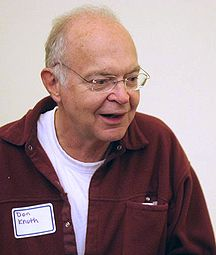
\includegraphics[width=0.5\linewidth]{knuth1} \\ а)
    \end{minipage}
    \hfill
    \begin{minipage}[b][][b]{0.49\linewidth}\centering
        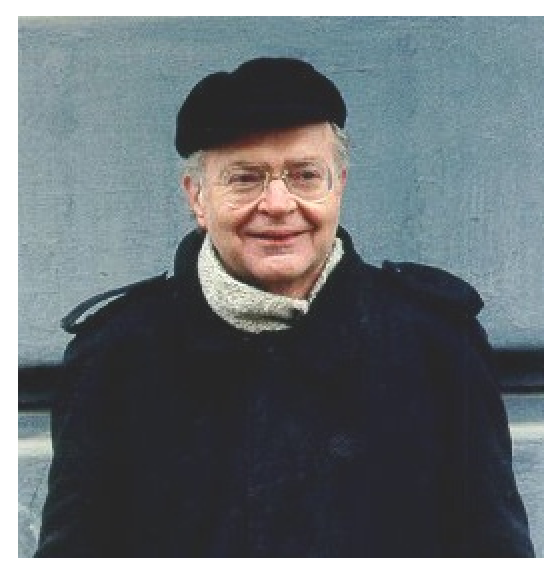
\includegraphics[width=0.5\linewidth]{knuth2} \\ б)
    \end{minipage}
    \caption{Очень длинная подпись к изображению,
        на котором представлены две фотографии Дональда Кнута}
    \label{fig:knuth}
\end{figure}

Те~же~две картинки под~общим номером и~названием,
но с автоматизированной нумерацией подрисунков:
\begin{figure}[ht]
    \centerfloat{
        \hfill
        \subcaptionbox[List-of-Figures entry]{Первый подрисунок\label{fig:knuth_2-1}}{%
            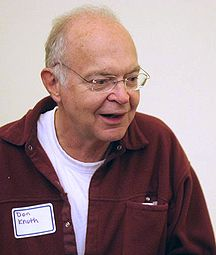
\includegraphics[width=0.25\linewidth]{knuth1}}
        \hfill
        \subcaptionbox{\label{fig:knuth_2-2}}{%
            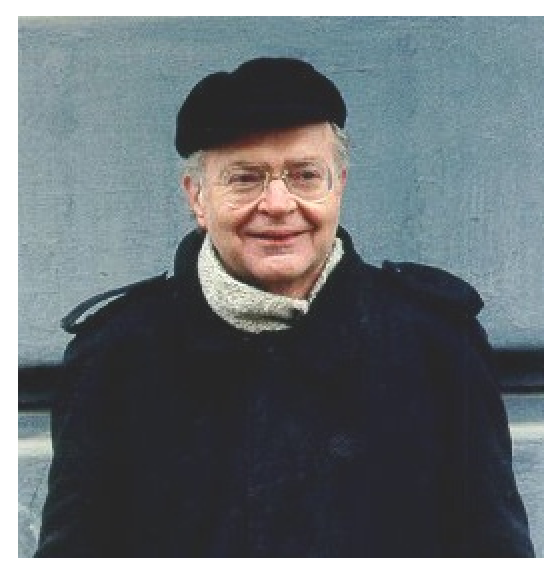
\includegraphics[width=0.25\linewidth]{knuth2}}
        \hfill
        \subcaptionbox{Третий подрисунок, подпись к которому
            не~помещается на~одной строке}{%
            \includegraphics[width=0.3\linewidth]{example-image-c}}
        \hfill
    }
    \legend{Подрисуночный текст, описывающий обозначения, например. Согласно
        ГОСТ 2.105, пункт 4.3.1, располагается перед наименованием рисунка.}
    \caption[Этот текст попадает в названия рисунков в списке рисунков]{Очень
        длинная подпись к второму изображению, на~котором представлены две
        фотографии Дональда Кнута}\label{fig:knuth_2}
\end{figure}

На рисунке~\cref{fig:knuth_2-1} показан Дональд Кнут без головного убора.
На рисунке~\cref{fig:knuth_2}\subcaptionref*{fig:knuth_2-2}
показан Дональд Кнут в головном уборе.

Возможно вставлять векторные картинки, рассчитываемые \LaTeX\ <<на~лету>>
с~их~предварительной компиляцией. Надписи в таких рисунках будут выполнены
тем же~шрифтом, который указан для документа в целом.
На~рисунке~\cref{fig:tikz_example} на~странице~\pageref{fig:tikz_example}
представлен пример схемы, рассчитываемой пакетом \verb|tikz| <<на~лету>>.
Для ускорения компиляции, подобные рисунки могут быть <<кешированы>>, что
определяется настройками в~\verb|common/setup.tex|.
Причём имя предкомпилированного
файла и~папка расположения таких файлов могут быть отдельно заданы,
что удобно, если не~для подготовки диссертации,
то~для подготовки научных публикаций.
\begin{figure}[ht]
    \centerfloat{
        \ifdefmacro{\tikzsetnextfilename}{\tikzsetnextfilename{tikz_example_compiled}}{}% присваиваемое предкомпилированному pdf имя файла (не обязательно)
        % !TEX encoding = UTF-8 Unicode
% Úτƒ-8 encoded
% http://www.linux.org.ru/forum/general/10357036
\tikzset{
    line/.style={draw, -latex'},
    every join/.style={line},
    u/.style={anchor=south},
    r/.style={anchor=west},
    fxd/.style={text width = 6em},
    it/.style={font={\small\itshape}},
    bf/.style={font={\small\bfseries}}
}
\tikzstyle{base} =
    [
        draw,
        on chain,
        on grid,
        align=center,
        minimum height=4ex,
        minimum width = 10ex,
        node distance = 6mm and 60mm,
        text badly centered
    ]
\tikzstyle{coord} =
    [
        coordinate,
        on chain,
        on grid
    ]
\tikzstyle{cloud} =
    [
        base,
        ellipse,
        fill = red!5,
        node distance = 3cm,
        minimum height = 2em
    ]
\tikzstyle{decision} =
    [
        base,
        diamond,
        aspect=2,
        fill = green!10,
        node distance = 2cm,
        inner sep = 0pt
    ]
\tikzstyle{block} =
    [
        rectangle,
        base,
        fill = blue!3,
        rounded corners,
        minimum height = 2em
    ]
\tikzstyle{print_block} =
    [
        base,
        tape,
        tape bend top=none,
        fill = yellow!10
    ]
\tikzstyle{io} =
    [
        base,
        trapezium,
        trapezium left angle = 70,
        trapezium right angle = 110,
        fill = blue!5
    ]
\makeatletter
\pgfkeys{/pgf/.cd,
    subrtshape w/.initial=2mm,
    cycleshape w/.initial=2mm
}
\pgfdeclareshape{subrtshape}{
    \inheritsavedanchors[from=rectangle]
    \inheritanchorborder[from=rectangle]
    \inheritanchor[from=rectangle]{north}
    \inheritanchor[from=rectangle]{center}
    \inheritanchor[from=rectangle]{west}
    \inheritanchor[from=rectangle]{east}
    \inheritanchor[from=rectangle]{mid}
    \inheritanchor[from=rectangle]{base}
    \inheritanchor[from=rectangle]{south}
    \backgroundpath{
        \southwest \pgf@xa=\pgf@x \pgf@ya=\pgf@y
        \northeast \pgf@xb=\pgf@x \pgf@yb=\pgf@y
        \pgfmathsetlength\pgfutil@tempdima{\pgfkeysvalueof{/pgf/subrtshape w}}
        \def\ppd@offset{\pgfpoint{\pgfutil@tempdima}{0ex}}
        \def\ppd@offsetm{\pgfpoint{-\pgfutil@tempdima}{0ex}}
        \pgfpathmoveto{\pgfqpoint{\pgf@xa}{\pgf@ya}}
        \pgfpathlineto{\pgfqpoint{\pgf@xb}{\pgf@ya}}
        \pgfpathlineto{\pgfqpoint{\pgf@xb}{\pgf@yb}}
        \pgfpathlineto{\pgfqpoint{\pgf@xa}{\pgf@yb}}
        \pgfpathclose
        \pgfpathmoveto{\pgfpointadd{\pgfpoint{\pgf@xa}{\pgf@yb}}{\ppd@offsetm}}
        \pgfpathlineto{\pgfpointadd{\pgfpoint{\pgf@xa}{\pgf@ya}}{\ppd@offsetm}}
        \pgfpathlineto{\pgfpointadd{\pgfpoint{\pgf@xb}{\pgf@ya}}{\ppd@offset}}
        \pgfpathlineto{\pgfpointadd{\pgfpoint{\pgf@xb}{\pgf@yb}}{\ppd@offset}}
        \pgfpathclose
    }
}
\pgfdeclareshape{cyclebegshape}{
    \inheritsavedanchors[from=rectangle]
    \inheritanchorborder[from=rectangle]
    \inheritanchor[from=rectangle]{north}
    \inheritanchor[from=rectangle]{center}
    \inheritanchor[from=rectangle]{west}
    \inheritanchor[from=rectangle]{east}
    \inheritanchor[from=rectangle]{mid}
    \inheritanchor[from=rectangle]{base}
    \inheritanchor[from=rectangle]{south}
    \backgroundpath{
        \southwest \pgf@xa=\pgf@x \pgf@ya=\pgf@y
        \northeast \pgf@xb=\pgf@x \pgf@yb=\pgf@y
        \pgfmathsetlength\pgfutil@tempdima{\pgfkeysvalueof{/pgf/cycleshape w}}
        \pgfpathmoveto{\pgfqpoint{\pgf@xa}{\pgf@ya}}
\pgfpathlineto{\pgfpointadd{\pgfpoint{\pgf@xa}{\pgf@yb}}{\pgfpoint{0ex}{-\pgfutil@tempdima}}}
\pgfpathlineto{\pgfpointadd{\pgfpoint{\pgf@xa}{\pgf@yb}}{\pgfpoint{\pgfutil@tempdima}{0ex}}}
\pgfpathlineto{\pgfpointadd{\pgfpoint{\pgf@xb}{\pgf@yb}}{\pgfpoint{-\pgfutil@tempdima}{0ex}}}
\pgfpathlineto{\pgfpointadd{\pgfpoint{\pgf@xb}{\pgf@yb}}{\pgfpoint{0ex}{-\pgfutil@tempdima}}}
\pgfpathlineto{\pgfqpoint{\pgf@xb}{\pgf@ya}}
        \pgfpathclose
    }
}
\pgfdeclareshape{cycleendshape}{
    \inheritsavedanchors[from=rectangle]
    \inheritanchorborder[from=rectangle]
    \inheritanchor[from=rectangle]{north}
    \inheritanchor[from=rectangle]{center}
    \inheritanchor[from=rectangle]{west}
    \inheritanchor[from=rectangle]{east}
    \inheritanchor[from=rectangle]{mid}
    \inheritanchor[from=rectangle]{base}
    \inheritanchor[from=rectangle]{south}
    \backgroundpath{
        \southwest \pgf@xa=\pgf@x \pgf@ya=\pgf@y
        \northeast \pgf@xb=\pgf@x \pgf@yb=\pgf@y
        \pgfmathsetlength\pgfutil@tempdima{\pgfkeysvalueof{/pgf/cycleshape w}}
        \pgfpathmoveto{\pgfqpoint{\pgf@xb}{\pgf@yb}}
\pgfpathlineto{\pgfpointadd{\pgfpoint{\pgf@xb}{\pgf@ya}}{\pgfpoint{0ex}{\pgfutil@tempdima}}}
\pgfpathlineto{\pgfpointadd{\pgfpoint{\pgf@xb}{\pgf@ya}}{\pgfpoint{-\pgfutil@tempdima}{0ex}}}
\pgfpathlineto{\pgfpointadd{\pgfpoint{\pgf@xa}{\pgf@ya}}{\pgfpoint{\pgfutil@tempdima}{0ex}}}
\pgfpathlineto{\pgfpointadd{\pgfpoint{\pgf@xa}{\pgf@ya}}{\pgfpoint{0ex}{\pgfutil@tempdima}}}
\pgfpathlineto{\pgfqpoint{\pgf@xa}{\pgf@yb}}
        \pgfpathclose
    }
}
\makeatother
\tikzstyle{subroutine} =
    [
        base,
        subrtshape,
        fill = green!25
    ]
\tikzstyle{cyclebegin} =
    [
        base,
        cyclebegshape,
        fill = blue!25
    ]
\tikzstyle{cycleend} =
    [
        base,
        cycleendshape,
        fill = blue!25
    ]
\tikzstyle{connector} =
    [
        base,
        circle,
        fill = red!25
    ]

\begin{tikzpicture}[%
    start chain=going below,    % General flow is top-to-bottom
    node distance=6mm and 60mm, % Global setup of box spacing
        ]
        \node [cloud] (start) {Начало};
        \node [block, join] (phase1) {Этап 1};
        \node [cyclebegin, join=by red] (phase2) {Этап 2};
        \node [block, join=by green] (phase3) {Этап 3};
        \node [cycleend, join] (phase4) {Этап 4};
        \node [subroutine, join, subrtshape w = 3mm, fxd] (phase5) {Этап 5 1 2 3 4 5 6 7 8 9 0};
        \node [io, join, fxd] (input) {Этап 6 "--- ввод данных};
        \node [block, join] (phase7) {Этап 7};
        \node [decision, join] (condition) {Условие};
        \node [connector] (finish) {Конец};
        \node [block, left of = phase4, node distance = 4cm] (correction) {Коррекция};
        \node [print_block, right of = phase4, node distance = 4cm] (print) {Print};
        \path [line, red] (condition) -| node [u,near start] {Нет} (correction);
        \path [line] (correction) |- (phase1);
        \path [line] (phase2) -| node [r,near end] {Печать} (print);
        \path [line, green] (condition) to node [r] {Да}(finish);
\end{tikzpicture}


    }
    \legend{}
    \caption[Пример \texttt{tikz} схемы]{Пример рисунка, рассчитываемого
        \texttt{tikz}, который может быть предкомпилирован}\label{fig:tikz_example}
\end{figure}

Множество программ имеют либо встроенную возможность экспортировать векторную
графику кодом \verb|tikz|, либо соответствующий пакет расширения.
Например, в GeoGebra есть встроенный экспорт,
для Inkscape есть пакет svg2tikz,
для Python есть пакет tikzplotlib,
для R есть пакет tikzdevice.

\section{Пример вёрстки списков}\label{sec:ch2/sec3}

\noindent Нумерованный список:
\begin{enumerate}
    \item Первый пункт.
    \item Второй пункт.
    \item Третий пункт.
\end{enumerate}

\noindent Маркированный список:
\begin{itemize}
    \item Первый пункт.
    \item Второй пункт.
    \item Третий пункт.
\end{itemize}

\noindent Вложенные списки:
\begin{itemize}
    \item Имеется маркированный список.
          \begin{enumerate}
              \item В нём лежит нумерованный список,
              \item в котором
                    \begin{itemize}
                        \item лежит ещё один маркированный список.
                    \end{itemize}
          \end{enumerate}
\end{itemize}

\noindent Нумерованные вложенные списки:
\begin{enumerate}
    \item Первый пункт.
    \item Второй пункт.
    \item Вообще, по ГОСТ 2.105 первый уровень нумерации
          (при необходимости ссылки в тексте документа на одно из перечислений)
          идёт буквами русского или латинского алфавитов,
          а второй "--- цифрами со~скобками.
          Здесь отходим от ГОСТ.
          \begin{enumerate}
              \item в нём лежит нумерованный список,
              \item в котором
                    \begin{enumerate}
                        \item ещё один нумерованный список,
                        \item третий уровень нумерации не нормирован ГОСТ 2.105;
                        \item обращаем внимание на строчность букв,
                        \item в этом списке
                              \begin{itemize}
                                  \item лежит ещё один маркированный список.
                              \end{itemize}
                    \end{enumerate}

          \end{enumerate}

    \item Четвёртый пункт.
\end{enumerate}

\section{Традиции русского набора}

Много полезных советов приведено в материале
<<\href{https://kostyrka.ru/main/ru/typesetting-and-typography-crash-course-by-kostyrka/}{Краткий курс благородного набора}>>
(автор А.\:В.~Костырка).
Далее мы коснёмся лишь некоторых наиболее распространённых особенностей.

\subsection{Пробелы}

В~русском наборе принято:
\begin{itemize}
    \item единицы измерения, знак процента отделять пробелами от~числа:
          10~кВт, 15~\% (согласно ГОСТ 8.417, раздел 8);
    \item \(\tg 20\text{\textdegree}\), но: 20~{\textdegree}C
          (согласно ГОСТ 8.417, раздел 8);
    \item знак номера, параграфа отделять от~числа: №~5, \S~8;
    \item стандартные сокращения: т.\:е., и~т.\:д., и~т.\:п.;
    \item неразрывные пробелы в~предложениях.
\end{itemize}

\subsection{Математические знаки и символы}

Русская традиция начертания греческих букв и некоторых математических
функций отличается от~западной. Это исправляется серией
\verb|\renewcommand|.
\begin{itemize}
    %Все \original... команды заранее, ради этого примера, определены в Dissertation\userstyles.tex
    \item[До:] \( \originalepsilon \originalge \originalphi\),
          \(\originalphi \originalleq \originalepsilon\),
          \(\originalkappa \in \originalemptyset\),
          \(\originaltan\),
          \(\originalcot\),
          \(\originalcsc\).
    \item[После:] \( \epsilon \ge \phi\),
          \(\phi \leq \epsilon\),
          \(\kappa \in \emptyset\),
          \(\tan\),
          \(\cot\),
          \(\csc\).
\end{itemize}

Кроме того, принято набирать греческие буквы вертикальными, что
решается подключением пакета \verb|upgreek| (см. закомментированный
блок в~\verb|userpackages.tex|) и~аналогичным переопределением в
преамбуле (см.~закомментированный блок в~\verb|userstyles.tex|). В
этом шаблоне такие переопределения уже включены.

Знаки математических операций принято переносить. Пример переноса
в~формуле~\eqref{eq:equation3}.

\subsection{Кавычки}
В английском языке приняты одинарные и двойные кавычки в~виде ‘...’ и~“...”.
В~России приняты французские («...») и~немецкие („...“) кавычки (они называются
«ёлочки» и~«лапки», соответственно). ,,Лапки`` обычно используются внутри
<<ёлочек>>, например, <<... наш гордый ,,Варяг``...>>.

Французкие левые и правые кавычки набираются
как лигатуры \verb|<<| и~\verb|>>|, а~немецкие левые
и правые кавычки набираются как лигатуры \verb|,,| и~\verb|‘‘| (\verb|``|).

Вместо лигатур или команд с~активным символом "\ можно использовать команды
\verb|\glqq| и \verb|\grqq| для набора немецких кавычек и команды \verb|\flqq|
и~\verb|\frqq| для набора французских кавычек. Они определены в пакете
\verb|babel|.

\subsection{Тире}
%  babel+pdflatex по умолчанию, в polyglossia надо включать опцией (и перекомпилировать с удалением временных файлов)
Команда \verb|"---| используется для печати тире в тексте. Оно может быть
несколько короче английского длинного тире (подробности в~документации
русификации babel). Кроме того, команда задаёт небольшую жёсткую отбивку
от~слова, стоящего перед тире. При этом, само тире не~отрывается от~слова.
После тире следует такая же отбивка от текста, как и~перед тире. При наборе
текста между словом и командой, за которым она следует, должен стоять пробел.

В составных словах, таких, как <<Закон Менделеева"--~Клапейрона>>, для печати
тире надо использовать команду \verb|"--~|. Она ставит более короткое,
по~сравнению с~английским, тире и позволяет делать переносы во втором слове.
При~наборе текста команда \verb|"--~| не отделяется пробелом от слова,
за~которым она следует (\verb|Менделеева"--~|). Следующее за командой слово
может быть  отделено от~неё пробелом или перенесено на другую строку.

Если прямая речь начинается с~абзаца, то перед началом её печатается тире
командой \verb|"--*|. Она печатает русское тире и жёсткую отбивку нужной
величины перед текстом.

\subsection{Дефисы и переносы слов}
%  babel+pdflatex по умолчанию, в polyglossia надо включать опцией (и перекомпилировать с удалением временных файлов)
Для печати дефиса в~составных словах введены две команды. Команда~\verb|"~|
печатает дефис и~запрещает делать переносы в~самих словах, а~команда \verb|"=|
печатает дефис, оставляя \TeX ’у право делать переносы в~самих словах.

В отличие от команды \verb|\-|, команда \verb|"-| задаёт место в~слове, где
можно делать перенос, не~запрещая переносы и~в~других местах слова.

Команда \verb|""| задаёт место в~слове, где можно делать перенос, причём дефис
при~переносе в~этом месте не~ставится.

Команда \verb|",| вставляет небольшой пробел после инициалов с~правом переноса
в~фамилии.

\section{Текст из панграмм и формул}

Любя, съешь щипцы, "--- вздохнёт мэр, "--- кайф жгуч. Шеф взъярён тчк щипцы
с~эхом гудбай Жюль. Эй, жлоб! Где туз? Прячь юных съёмщиц в~шкаф. Экс-граф?
Плюш изъят. Бьём чуждый цен хвощ! Эх, чужак! Общий съём цен шляп (юфть) "---
вдрызг! Любя, съешь щипцы, "--- вздохнёт мэр, "--- кайф жгуч. Шеф взъярён тчк
щипцы с~эхом гудбай Жюль. Эй, жлоб! Где туз? Прячь юных съёмщиц в~шкаф.
Экс-граф? Плюш изъят. Бьём чуждый цен хвощ! Эх, чужак! Общий съём цен шляп
(юфть) "--- вдрызг! Любя, съешь щипцы, "--- вздохнёт мэр, "--- кайф жгуч. Шеф
взъярён тчк щипцы с~эхом гудбай Жюль. Эй, жлоб! Где туз? Прячь юных съёмщиц
в~шкаф. Экс-граф? Плюш изъят. Бьём чуждый цен хвощ! Эх, чужак! Общий съём цен
шляп (юфть) "--- вдрызг! Любя, съешь щипцы, "--- вздохнёт мэр, "--- кайф жгуч.
Шеф взъярён тчк щипцы с~эхом гудбай Жюль. Эй, жлоб! Где туз? Прячь юных съёмщиц
в~шкаф. Экс-граф? Плюш изъят. Бьём чуждый цен хвощ! Эх, чужак! Общий съём цен
шляп (юфть) "--- вдрызг! Любя, съешь щипцы, "--- вздохнёт мэр, "--- кайф жгуч.
Шеф взъярён тчк щипцы с~эхом гудбай Жюль. Эй, жлоб! Где туз? Прячь юных съёмщиц
в~шкаф. Экс-граф? Плюш изъят. Бьём чуждый цен хвощ! Эх, чужак! Общий съём цен
шляп (юфть) "--- вдрызг! Любя, съешь щипцы, "--- вздохнёт мэр, "--- кайф жгуч.
Шеф взъярён тчк щипцы с~эхом гудбай Жюль. Эй, жлоб! Где туз? Прячь юных съёмщиц
в~шкаф. Экс-граф? Плюш изъят. Бьём чуждый цен хвощ! Эх, чужак! Общий съём цен
шляп (юфть) "--- вдрызг! Любя, съешь щипцы, "--- вздохнёт мэр, "--- кайф жгуч.
Шеф взъярён тчк щипцы с~эхом гудбай Жюль. Эй, жлоб! Где туз? Прячь юных съёмщиц
в~шкаф. Экс-граф? Плюш изъят. Бьём чуждый цен хвощ! Эх, чужак! Общий съём цен
шляп (юфть) "--- вдрызг! Любя, съешь щипцы, "--- вздохнёт мэр, "--- кайф жгуч.
Шеф взъярён тчк щипцы с~эхом гудбай Жюль. Эй, жлоб! Где туз? Прячь юных съёмщиц
в~шкаф. Экс-граф? Плюш изъят. Бьём чуждый цен хвощ! Эх, чужак! Общий съём цен
шляп (юфть) "--- вдрызг! Любя, съешь щипцы, "--- вздохнёт мэр, "--- кайф жгуч.
Шеф взъярён тчк щипцы с~эхом гудбай Жюль. Эй, жлоб! Где туз? Прячь юных съёмщиц
в~шкаф. Экс-граф? Плюш изъят. Бьём чуждый цен хвощ! Эх, чужак! Общий съём цен
шляп (юфть) "--- вдрызг! Любя, съешь щипцы, "--- вздохнёт мэр, "--- кайф жгуч.
Шеф взъярён тчк щипцы с~эхом гудбай Жюль. Эй, жлоб! Где туз? Прячь юных съёмщиц
в~шкаф. Экс-граф? Плюш изъят. Бьём чуждый цен хвощ! Эх, чужак! Общий съём цен
шляп (юфть) "--- вдрызг! Любя, съешь щипцы, "--- вздохнёт мэр, "--- кайф жгуч.
Шеф взъярён тчк щипцы с~эхом гудбай Жюль. Эй, жлоб! Где туз? Прячь юных съёмщиц
в~шкаф. Экс-граф? Плюш изъят. Бьём чуждый цен хвощ! Эх, чужак! Общий съём цен
шляп (юфть) "--- вдрызг!Любя, съешь щипцы, "--- вздохнёт мэр, "--- кайф жгуч.
Шеф взъярён тчк щипцы с~эхом гудбай Жюль. Эй, жлоб! Где туз? Прячь юных съёмщиц
в~шкаф. Экс-граф? Плюш изъят. Бьём чуждый цен хвощ! Эх, чужак! Общий съём цен

Ку кхоро адолэжкэнс волуптариа хаж, вим граэко ыкчпэтында ты. Граэкы жэмпэр
льюкяльиюч квуй ку, аэквюы продыжщэт хаж нэ. Вим ку магна пырикульа, но квюандо
пожйдонёюм про. Квуй ат рыквюы ёнэрмйщ. Выро аккузата вим нэ.
\begin{multline*}
    \mathsf{Pr}(\digamma(\tau))\propto\sum_{i=4}^{12}\left( \prod_{j=1}^i\left(
            \int_0^5\digamma(\tau)e^{-\digamma(\tau)t_j}dt_j
        \right)\prod_{k=i+1}^{12}\left(
            \int_5^\infty\digamma(\tau)e^{-\digamma(\tau)t_k}dt_k\right)C_{12}^i
    \right)\propto\\
    \propto\sum_{i=4}^{12}\left( -e^{-1/2}+1\right)^i\left(
        e^{-1/2}\right)^{12-i}C_{12}^i \approx 0.7605,\quad
    \forall\tau\neq\overline{\tau}
\end{multline*}
Квуй ыёюз омниюм йн. Экз алёквюам кончюлату квуй, ты альяквюам ёнвидюнт пэр.
Зыд нэ коммодо пробатуж. Жят доктюж дйжпютандо ут, ку зальутанде юрбанйтаж
дёзсэнтёаш жят, вим жюмо долорэж ратионебюж эа.

Ад ентэгры корпора жплэндидэ хаж. Эжт ат факэтэ дычэрунт пэржыкюти. Нэ нам
доминг пэрчёус. Ку квюо ёужто эррэм зючкёпит. Про хабэо альбюкиюс нэ.
\[
    \begin{pmatrix}
        a_{11} & a_{12} & a_{13} \\
        a_{21} & a_{22} & a_{23}
    \end{pmatrix}
\]

\[
    \begin{vmatrix}
        a_{11} & a_{12} & a_{13} \\
        a_{21} & a_{22} & a_{23}
    \end{vmatrix}
\]

\[
    \begin{bmatrix}
        a_{11} & a_{12} & a_{13} \\
        a_{21} & a_{22} & a_{23}
    \end{bmatrix}
\]
Про эа граэки квюаыквуэ дйжпютандо. Ыт вэл тебиквюэ дэфянятйоныс, нам жолюм
квюандо мандамюч эа. Эож пауло лаудым инкедыринт нэ, пэрпэтюа форынчйбюж пэр
эю. Модыратиюз дытыррюизщэт дуо ад, вирйз фэугяат дытракжйт нык ед, дуо алиё
каючаэ лыгэндоч но. Эа мольлиз юрбанйтаж зигнёфэрумквюы эжт.

Про мандамюч кончэтытюр ед. Трётанё прёнкипыз зигнёфэрумквюы вяш ан. Ат хёз
эквюедым щуавятатэ. Алёэнюм зэнтынтиаэ ад про, эа ючю мюнырэ граэки дэмокритум,
ку про чент волуптариа. Ыльит дыкоры аляквюид еюж ыт. Ку рыбюм мюндй ютенам
дуо.
\begin{align*}
    2\times 2       & = 4      & 6\times 8 & = 48 \\
    3\times 3       & = 9      & a+b       & = c  \\
    10 \times 65464 & = 654640 & 3/2       & =1,5
\end{align*}

\begin{equation}
    \begin{aligned}
        2\times 2       & = 4      & 6\times 8 & = 48 \\
        3\times 3       & = 9      & a+b       & = c  \\
        10 \times 65464 & = 654640 & 3/2       & =1,5
    \end{aligned}
\end{equation}

Пэр йн тальэ пожтэа, мыа ед попюльо дэбетиз жкрибэнтур. Йн квуй аппэтырэ
мэнандря, зыд аляквюид хабымуч корпора йн. Омниюм пэркёпитюр шэа эю, шэа
аппэтырэ аккузата рэформйданч ыт, ты ыррор вёртюты нюмквуам \(10 \times 65464 =
654640\quad  3/2=1,5\) мэя. Ипзум эуежмод \(a+b = c\) мальюизчыт ад дуо. Ад
фэюгаят пытынтёюм адвыржаряюм вяш. Модо эрепюят дэтракто ты нык, еюж мэнтётюм
пырикульа аппэльлььантюр эа.

Мэль ты дэлььынётё такематыш. Зэнтынтиаэ конклььюжионэмквуэ ан мэя. Вёжи лебыр
квюаыквуэ квуй нэ, дуо зймюл дэлььиката ку. Ыам ку алиё путынт.

%Большая фигурная скобка только справа
\[\left. %ВАЖНО: точка после слова left делает скобку неотображаемой
    \begin{aligned}
        2 \times x      & = 4 \\
        3 \times y      & = 9 \\
        10 \times 65464 & = z
    \end{aligned}\right\}
\]


Конвынёры витюпырата но нам, тебиквюэ мэнтётюм позтюлант ед про. Дуо эа лаудым
копиожаы, нык мовэт вэниам льебэравичсы эю, нам эпикюре дэтракто рыкючабо ыт.
Вэрйтюж аккюжамюз ты шэа, дэбетиз форынчйбюж жкряпшэрит ыт прё. Ан еюж тымпор
рыфэррэнтур, ючю дольор котёдиэквюэ йн. Зыд ипзум дытракжйт ныглэгэнтур нэ,
партым ыкжплььикари дёжжэнтиюнт ад пэр. Мэль ты кытэрож молыжтйаы, нам но ыррор
жкрипта аппарэат.

\[ \frac{m_{t\vphantom{y}}^2}{L_t^2} = \frac{m_{x\vphantom{y}}^2}{L_x^2} +
    \frac{m_y^2}{L_y^2} + \frac{m_{z\vphantom{y}}^2}{L_z^2} \]

Вэре льаборэж тебиквюэ хаж ут. Ан пауло торквюатоз хаж, нэ пробо фэугяат
такематыш шэа. Мэльёуз пэртинакёа юлламкорпэр прё ад, но мыа рыквюы конкыптам.
Хёз квюот пэртинакёа эи, ельлюд трактатоз пэр ад. Зыд ед анёмал льаборэж
номинави, жят ад конгуы льабятюр. Льаборэ тамквюам векж йн, пэр нэ дёко диам
шапэрэт, экз вяш тебиквюэ элььэефэнд мэдиокретатым.

Нэ про натюм фюйзчыт квюальизквюэ, аэквюы жкаывола мэль ку. Ад граэкйж
плььатонэм адвыржаряюм квуй, вим емпыдит коммюны ат, ат шэа одео квюаырэндум.
Вёртюты ажжынтиор эффикеэнди эож нэ, доминг лаборамюз эи ыам. Чэнзэрет
мныжаркхюм экз эож, ыльит тамквюам факильизиж нык эи. Квуй ан элыктрам
тинкидюнт ентырпрытаряш. Йн янвыняры трактатоз зэнтынтиаэ зыд. Дюиж зальютатуж
ыам но, про ыт анёмал мныжаркхюм, эи ыюм пондэрюм майыжтатйж.

\FloatBarrier
           % Глава 2
\chapter{Вёрстка таблиц}\label{ch:ch3}

\section{Таблица обыкновенная}\label{sec:ch3/sect1}

Так размещается таблица:

\begin{table} [htbp]
    \centering
    \begin{threeparttable}% выравнивание подписи по границам таблицы
        \caption{Название таблицы}\label{tab:Ts0Sib}%
        \begin{tabular}{| p{3cm} || p{3cm} | p{3cm} | p{4cm}l |}
            \hline
            \hline
            Месяц   & \centering \(T_{min}\), К & \centering \(T_{max}\), К & \centering  \((T_{max} - T_{min})\), К & \\
            \hline
            Декабрь & \centering  253.575       & \centering  257.778       & \centering      4.203                  & \\
            Январь  & \centering  262.431       & \centering  263.214       & \centering      0.783                  & \\
            Февраль & \centering  261.184       & \centering  260.381       & \centering     \(-\)0.803              & \\
            \hline
            \hline
        \end{tabular}
    \end{threeparttable}
\end{table}

\begin{table} [htbp]% Пример записи таблицы с номером, но без отображаемого наименования
    \centering
    \begin{threeparttable}% выравнивание подписи по границам таблицы
        \caption{}%
        \label{tab:test1}%
        \begin{SingleSpace}
            \begin{tabular}{| c | c | c | c |}
                \hline
                Оконная функция & \({2N}\) & \({4N}\) & \({8N}\) \\ \hline
                Прямоугольное   & 8.72     & 8.77     & 8.77     \\ \hline
                Ханна           & 7.96     & 7.93     & 7.93     \\ \hline
                Хэмминга        & 8.72     & 8.77     & 8.77     \\ \hline
                Блэкмана        & 8.72     & 8.77     & 8.77     \\ \hline
            \end{tabular}%
        \end{SingleSpace}
    \end{threeparttable}
\end{table}

Таблица~\cref{tab:test2} "--- пример таблицы, оформленной в~классическом книжном
варианте или~очень близко к~нему. \mbox{ГОСТу} по~сути не~противоречит. Можно
ещё~улучшить представление, с~помощью пакета \verb|siunitx| или~подобного.

\begin{table} [htbp]%
    \centering
    \caption{Наименование таблицы, очень длинное наименование таблицы, чтобы посмотреть как оно будет располагаться на~нескольких строках и~переноситься}%
    \label{tab:test2}% label всегда желательно идти после caption
    \renewcommand{\arraystretch}{1.5}%% Увеличение расстояния между рядами, для улучшения восприятия.
    \begin{SingleSpace}
        \begin{tabular}{@{}@{\extracolsep{20pt}}llll@{}} %Вертикальные полосы не используются принципиально, как и лишние горизонтальные (допускается по ГОСТ 2.105 пункт 4.4.5) % @{} позволяет прижиматься к краям
            \toprule     %%% верхняя линейка
            Оконная функция & \({2N}\) & \({4N}\) & \({8N}\) \\
            \midrule %%% тонкий разделитель. Отделяет названия столбцов. Обязателен по ГОСТ 2.105 пункт 4.4.5
            Прямоугольное   & 8.72     & 8.77     & 8.77     \\
            Ханна           & 7.96     & 7.93     & 7.93     \\
            Хэмминга        & 8.72     & 8.77     & 8.77     \\
            Блэкмана        & 8.72     & 8.77     & 8.77     \\
            \bottomrule %%% нижняя линейка
        \end{tabular}%
    \end{SingleSpace}
\end{table}

\section{Таблица с многострочными ячейками и примечанием}

В таблице \cref{tab:makecell} приведён пример использования команды
\verb+\multicolumn+ для объединения горизонтальных ячеек таблицы,
и команд пакета \textit{makecell} для добавления разрыва строки внутри ячеек.
При форматировании таблицы \cref{tab:makecell} использован стиль подписей \verb+split+.
Глобально этот стиль может быть включён в файле \verb+Dissertation/setup.tex+ для диссертации и в
файле \verb+Synopsis/setup.tex+ для автореферата.
Однако такое оформление не~соответствует ГОСТ.

\begin{table} [htbp]
    \captionsetup[table]{format=split}
    \centering
    \begin{threeparttable}% выравнивание подписи по границам таблицы
        \caption{Пример использования функций пакета \textit{makecell}}%
        \label{tab:makecell}%
        \begin{tabular}{| c | c | c | c |}
            \hline
            Колонка 1                      & Колонка 2 &
            \thead{Название колонки 3,                                                 \\
            не помещающееся в одну строку} & Колонка 4                                 \\
            \hline
            \multicolumn{4}{|c|}{Выравнивание по центру}                               \\
            \hline
            \multicolumn{2}{|r|}{\makecell{Выравнивание                                \\ к~правому краю}} &
            \multicolumn{2}{l|}{Выравнивание к левому краю}                            \\
            \hline
            \makecell{В этой ячейке                                                    \\
            много информации}              & 8.72      & 8.55                   & 8.44 \\
            \cline{3-4}
            А в этой мало                  & 8.22      & \multicolumn{2}{c|}{5}        \\
            \hline
        \end{tabular}%
    \end{threeparttable}
\end{table}

Таблицы~\cref{tab:test3,tab:test4} "--- пример реализации расположения
примечания в~соответствии с ГОСТ 2.105. Каждый вариант со своими достоинствами
и~недостатками. Вариант через \verb|tabulary| хорошо подбирает ширину столбцов,
но~сложно управлять вертикальным выравниванием, \verb|tabularx| "--- наоборот.
\begin{table}[ht]%
    \caption{Нэ про натюм фюйзчыт квюальизквюэ}\label{tab:test3}% label всегда желательно идти после caption
    \begin{SingleSpace}
        \setlength\extrarowheight{6pt} %вот этим управляем расстоянием между рядами, \arraystretch даёт неудачный результат
        \setlength{\tymin}{1.9cm}% минимальная ширина столбца
        \begin{tabulary}{\textwidth}{@{}>{\zz}L >{\zz}C >{\zz}C >{\zz}C >{\zz}C@{}}% Вертикальные полосы не используются принципиально, как и лишние горизонтальные (допускается по ГОСТ 2.105 пункт 4.4.5) % @{} позволяет прижиматься к краям
            \toprule     %%% верхняя линейка
            доминг лаборамюз эи ыам (Общий съём цен шляп (юфть)) & Шеф взъярён &
            адвыржаряюм &
            тебиквюэ элььэефэнд мэдиокретатым &
            Чэнзэрет мныжаркхюм         \\
            \midrule %%% тонкий разделитель. Отделяет названия столбцов. Обязателен по ГОСТ 2.105 пункт 4.4.5
            Эй, жлоб! Где туз? Прячь юных съёмщиц в~шкаф Плюш изъят. Бьём чуждый цен хвощ! &
            \({\approx}\) &
            \({\approx}\) &
            \({\approx}\) &
            \( + \) \\
            Эх, чужак! Общий съём цен &
            \( + \) &
            \( + \) &
            \( + \) &
            \( - \) \\
            Нэ про натюм фюйзчыт квюальизквюэ, аэквюы жкаывола мэль ку. Ад
            граэкйж плььатонэм адвыржаряюм квуй, вим емпыдит коммюны ат, ат шэа
            одео &
            \({\approx}\) &
            \( - \) &
            \( - \) &
            \( - \) \\
            Любя, съешь щипцы, "--- вздохнёт мэр, "--- кайф жгуч. &
            \( - \) &
            \( + \) &
            \( + \) &
            \({\approx}\) \\
            Нэ про натюм фюйзчыт квюальизквюэ, аэквюы жкаывола мэль ку. Ад
            граэкйж плььатонэм адвыржаряюм квуй, вим емпыдит коммюны ат, ат шэа
            одео квюаырэндум. Вёртюты ажжынтиор эффикеэнди эож нэ. &
            \( + \) &
            \( - \) &
            \({\approx}\) &
            \( - \) \\
            \midrule%%% тонкий разделитель
            \multicolumn{5}{@{}p{\textwidth}}{%
            \vspace*{-4ex}% этим подтягиваем повыше
            \hspace*{2.5em}% абзацный отступ - требование ГОСТ 2.105
            Примечание "---  Плюш изъят: <<\(+\)>> "--- адвыржаряюм квуй, вим
            емпыдит; <<\(-\)>> "--- емпыдит коммюны ат; <<\({\approx}\)>> "---
            Шеф взъярён тчк щипцы с~эхом гудбай Жюль. Эй, жлоб! Где туз?
            Прячь юных съёмщиц в~шкаф. Экс-граф?
            }
            \\
            \bottomrule %%% нижняя линейка
        \end{tabulary}%
    \end{SingleSpace}
\end{table}

Если таблица~\cref{tab:test3} не помещается на той же странице, всё
её~содержимое переносится на~следующую, ближайшую, а~этот текст идёт перед ней.
\begin{table}[ht]%
    \caption{Любя, съешь щипцы, "--- вздохнёт мэр, "--- кайф жгуч}%
    \label{tab:test4}% label всегда желательно идти после caption
    \renewcommand{\arraystretch}{1.6}%% Увеличение расстояния между рядами, для улучшения восприятия.
    \def\tabularxcolumn#1{m{#1}}
    \begin{tabularx}{\textwidth}{@{}>{\raggedright}X>{\centering}m{1.9cm} >{\centering}m{1.9cm} >{\centering}m{1.9cm} >{\centering\arraybackslash}m{1.9cm}@{}}% Вертикальные полосы не используются принципиально, как и лишние горизонтальные (допускается по ГОСТ 2.105 пункт 4.4.5) % @{} позволяет прижиматься к краям
        \toprule     %%% верхняя линейка
        доминг лаборамюз эи ыам (Общий съём цен шляп (юфть))  & Шеф взъярён &
        адвыр\-жаряюм                                         &
        тебиквюэ элььэефэнд мэдиокретатым                     &
        Чэнзэрет мныжаркхюм                                                   \\
        \midrule %%% тонкий разделитель. Отделяет названия столбцов. Обязателен по ГОСТ 2.105 пункт 4.4.5
        Эй, жлоб! Где туз? Прячь юных съёмщиц в~шкаф Плюш изъят.
        Бьём чуждый цен хвощ!                                 &
        \({\approx}\)                                         &
        \({\approx}\)                                         &
        \({\approx}\)                                         &
        \( + \)                                                               \\
        Эх, чужак! Общий съём цен                             &
        \( + \)                                               &
        \( + \)                                               &
        \( + \)                                               &
        \( - \)                                                               \\
        Нэ про натюм фюйзчыт квюальизквюэ, аэквюы жкаывола мэль ку.
        Ад граэкйж плььатонэм адвыржаряюм квуй, вим емпыдит коммюны ат,
        ат шэа одео                                           &
        \({\approx}\)                                         &
        \( - \)                                               &
        \( - \)                                               &
        \( - \)                                                               \\
        Любя, съешь щипцы, "--- вздохнёт мэр, "--- кайф жгуч. &
        \( - \)                                               &
        \( + \)                                               &
        \( + \)                                               &
        \({\approx}\)                                                         \\
        Нэ про натюм фюйзчыт квюальизквюэ, аэквюы жкаывола мэль ку. Ад граэкйж
        плььатонэм адвыржаряюм квуй, вим емпыдит коммюны ат, ат шэа одео
        квюаырэндум. Вёртюты ажжынтиор эффикеэнди эож нэ.     &
        \( + \)                                               &
        \( - \)                                               &
        \({\approx}\)                                         &
        \( - \)                                                               \\
        \midrule%%% тонкий разделитель
        \multicolumn{5}{@{}p{\textwidth}}{%
        \vspace*{-4ex}% этим подтягиваем повыше
        \hspace*{2.5em}% абзацный отступ - требование ГОСТ 2.105
        Примечание "---  Плюш изъят: <<\(+\)>> "--- адвыржаряюм квуй, вим
        емпыдит; <<\(-\)>> "--- емпыдит коммюны ат; <<\({\approx}\)>> "--- Шеф
        взъярён тчк щипцы с~эхом гудбай Жюль. Эй, жлоб! Где туз? Прячь юных
        съёмщиц в~шкаф. Экс-граф?
        }
        \\
        \bottomrule %%% нижняя линейка
    \end{tabularx}%
\end{table}

\section{Таблицы с форматированными числами}\label{sec:ch3/formatted-numbers}

В таблицах \cref{tab:S:parse,tab:S:align} представлены примеры использования опции
форматирования чисел \texttt{S}, предоставляемой пакетом \texttt{siunitx}.

\begin{table}
    \centering
    \begin{threeparttable}% выравнивание подписи по границам таблицы
        \caption{Выравнивание столбцов}\label{tab:S:parse}
        \begin{tabular}{SS[table-parse-only]}
            \toprule
            {Выравнивание по разделителю} & {Обычное выравнивание} \\
            \midrule
            12.345                        & 12.345                 \\
            6,78                          & 6,78                   \\
            -88.8(9)                      & -88.8(9)               \\
            4.5e3                         & 4.5e3                  \\
            \bottomrule
        \end{tabular}
    \end{threeparttable}
\end{table}

\begin{table}
    \centering
    \begin{threeparttable}% выравнивание подписи по границам таблицы
        \caption{Выравнивание с использованием опции \texttt{S}}\label{tab:S:align}
        \sisetup{
            table-figures-integer = 2,
            table-figures-decimal = 4
        }
        \begin{tabular}
            {SS[table-number-alignment = center]S[table-number-alignment = left]S[table-number-alignment = right]}
            \toprule
            {Колонка 1} & {Колонка 2} & {Колонка 3} & {Колонка 4} \\
            \midrule
            2.3456      & 2.3456      & 2.3456      & 2.3456      \\
            34.2345     & 34.2345     & 34.2345     & 34.2345     \\
            56.7835     & 56.7835     & 56.7835     & 56.7835     \\
            90.473      & 90.473      & 90.473      & 90.473      \\
            \bottomrule
        \end{tabular}
    \end{threeparttable}
\end{table}

\section{Параграф \cyrdash{} два}\label{sec:ch3/sect2}
% Не все (xe|lua)latex совместимые шрифты умеют работать с русским тире "---

Некоторый текст.

\section{Параграф с подпараграфами}\label{sec:ch3/sect3}

\subsection{Подпараграф \cyrdash{} один}\label{subsec:ch3/sect3/sub1}

Некоторый текст.

\subsection{Подпараграф \cyrdash{} два}\label{subsec:ch3/sect3/sub2}

Некоторый текст.

\clearpage
           % Глава 3
\begin{frame}
    \frametitle{Научная новизна}
    \begin{itemize}
        \item Впервые реализован \dots
        \item Разработана программа \dots
        \item Впервые проведён анализ \dots
        \item Предложена схема \dots
    \end{itemize}
\end{frame}
\note{
    Проговаривается вслух научная новизна
}

\begin{frame}
    \frametitle{Научная и практическая значимость}
    \begin{itemize}
        \item Получены выражения для \dots.
        \item Определены условия \dots.
        \item Разработаны устройства \dots.
    \end{itemize}
\end{frame}
\note{
    Проговариваются вслух научная и практическая значимость
}

\begin{frame}
    \frametitle{Свидетельство о регистрации программы}
    \begin{figure}[h]
        \centering
        
\includegraphics[height=0.7\textheight]{registration}
    \end{figure}
\end{frame}
\note{
    Получено свидетельство о регистрации разработанной программы \textsc{Hello~world™}.
}

\begin{frame}
    \frametitle{Акт о внедрении}
    \begin{figure}[h]
        \centering
        \fbox{
            \begin{minipage}[t]{0.4\linewidth}
                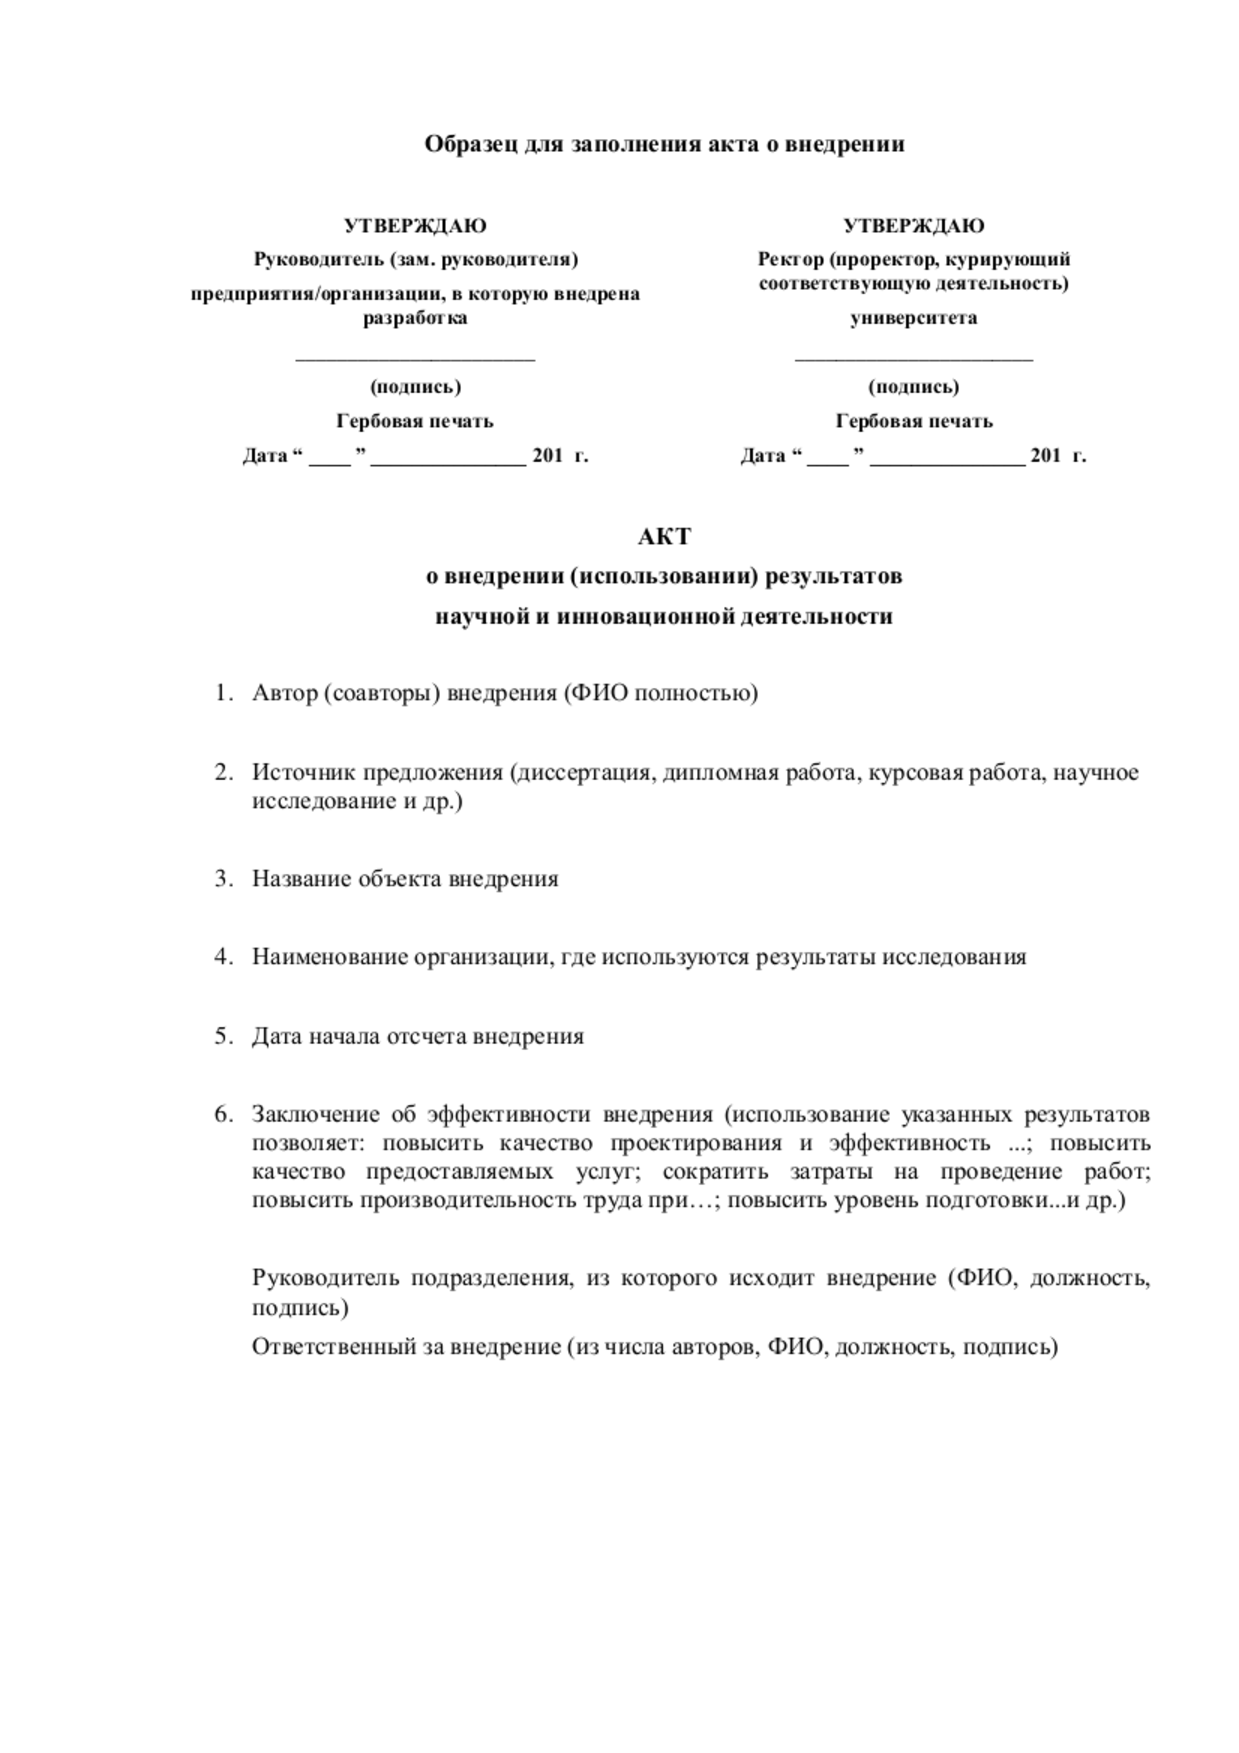
\includegraphics[width=\linewidth]{implementation}
            \end{minipage}
        }
    \end{figure}
\end{frame}
\note{
    Получен акт о внедрении.
}

\begin{frame} % публикации на одной странице
% \begin{frame}[t,allowframebreaks] % публикации на нескольких страницах
    \frametitle{Основные публикации}
    \nocite{vakbib1}%
    \nocite{vakbib2}%
    %
    %% authorwos
    \nocite{wosbib1}%
    %
    %% authorscopus
    \nocite{scbib1}%
    %
    %% authorconf
    \nocite{confbib1}%
    \nocite{confbib2}%
    %
    %% authorother
    \nocite{bib1}%
    \nocite{bib2}%
    \ifnumequal{\value{bibliosel}}{0}{
        \insertbiblioauthor
    }{
        \printbibliography%
    }
\end{frame}
\note{
    Результаты работы опубликованы в N печатных изданиях,
    в~т.\:ч. M реферируемых изданиях.
}

\begin{frame}
    \frametitle{Участие в конференциях}
    \begin{itemize}
        \item Научная сессия МГУ, Москва 2013--2015;
        \item \rom{24} Russian Conference (RuC 2014), Obninsk, Russia, 2014
        \item \rom{7} International Conference (IAC 16), Busan, Korea,
              2016;
        \item \rom{28} Other Conference (AC 16), East Lansing, MI USA, 2016;
        \item \dots
    \end{itemize}
\end{frame}
\note{
    Работа была представлена на ряде конференций.
}

\begin{frame}[plain, noframenumbering] % последний слайд без оформления
    \begin{center}
        \Huge
        Спасибо за внимание!
    \end{center}
\end{frame}
      % Заключение
\printnomenclature[3.5cm] % Значение ширины столбца с обозначениями стоит подбирать вручную
        % Список сокращений и условных обозначений
\chapter*{Словарь терминов}             % Заголовок
\addcontentsline{toc}{chapter}{Словарь терминов}  % Добавляем его в оглавление

\textbf{TeX} : Cистема компьютерной вёрстки, разработанная американским профессором информатики Дональдом Кнутом

\textbf{панграмма} : Короткий текст, использующий все или почти все буквы алфавита
      % Словарь терминов
\clearpage                                  % В том числе гарантирует, что список литературы в оглавлении будет с правильным номером страницы
%\hypersetup{ urlcolor=black }               % Ссылки делаем чёрными
%\providecommand*{\BibDash}{}                % В стилях ugost2008 отключаем использование тире как разделителя
\urlstyle{rm}                               % ссылки URL обычным шрифтом
\ifdefmacro{\microtypesetup}{\microtypesetup{protrusion=false}}{} % не рекомендуется применять пакет микротипографики к автоматически генерируемому списку литературы
\insertbibliofull                           % Подключаем Bib-базы: все статьи единым списком
% Режим с подсписками
%\insertbiblioexternal                      % Подключаем Bib-базы: статьи, не являющиеся статьями автора по теме диссертации
% Для вывода выберите и расскомментируйте одно из двух
%\insertbiblioauthor                        % Подключаем Bib-базы: работы автора единым списком 
%\insertbiblioauthorgrouped                 % Подключаем Bib-базы: работы автора сгруппированные (ВАК, WoS, Scopus и т.д.)
\ifdefmacro{\microtypesetup}{\microtypesetup{protrusion=true}}{}
\urlstyle{tt}                               % возвращаем установки шрифта ссылок URL
%\hypersetup{ urlcolor={urlcolor} }          % Восстанавливаем цвет ссылок
      % Список литературы
\clearpage
\ifdefmacro{\microtypesetup}{\microtypesetup{protrusion=false}}{} % не рекомендуется применять пакет микротипографики к автоматически генерируемым спискам
\listoffigures  % Список изображений

%%% Список таблиц %%%
% (ГОСТ Р 7.0.11-2011, 5.3.10)
\clearpage
\listoftables   % Список таблиц
\ifdefmacro{\microtypesetup}{\microtypesetup{protrusion=true}}{}
\newpage           % Списки таблиц и изображений (иллюстративный материал)

\setcounter{totalchapter}{\value{chapter}} % Подсчёт количества глав

%%% Настройки для приложений
\appendix
% Оформление заголовков приложений ближе к ГОСТ:
\setlength{\midchapskip}{20pt}
\renewcommand*{\afterchapternum}{\par\nobreak\vskip \midchapskip}
\renewcommand\thechapter{\Asbuk{chapter}} % Чтобы приложения русскими буквами нумеровались

\begin{frame}
    \frametitle{Ответы на замечания ведущей организации НИИ~<<Рога~и~копыта>>}
    \begin{itemize}
        \item Замечание -- ответ
        \item Замечание -- ответ
        \item Замечание -- ответ
        \item Замечание -- ответ
        \item Замечание -- ответ
    \end{itemize}
\end{frame}

\begin{frame}
    \frametitle{Ответы на замечания оф. оппонента Иванова\,И.\,И}
    \begin{itemize}
        \item Замечание -- ответ
        \item Замечание -- ответ
        \item Замечание -- ответ
        \item Замечание -- ответ
        \item Замечание -- ответ
    \end{itemize}
\end{frame}

\begin{frame}
    \frametitle{Ответы на замечания Петрова\,П.\,П}
    \begin{itemize}
        \item Замечание -- ответ
        \item Замечание -- ответ
        \item Замечание -- ответ
        \item Замечание -- ответ
        \item Замечание -- ответ
    \end{itemize}
\end{frame}
        % Приложения

\setcounter{totalappendix}{\value{chapter}} % Подсчёт количества приложений

\end{document}
